\chapter{Comparing three stochastic search algorithms for CPD}
\label{chap:Comparaison}


Ce chapitre reprend l'article publié dans \og Journal of Chemical Theory and Computation\fg \cite{Mignon16}.


\subsection*{Abstract}
Computational protein design depends on an energy function and an algorithm to search the sequence/conformation space.
We compare three stochastic search algorithms: a heuristic, Monte Carlo (MC), and a Replica Exchange Monte Carlo method (REMC).
The heuristic performs a steepest-descent minimization starting from thousands of random starting points.
The methods are applied to nine test proteins from three structural families, with a fixed backbone structure, a molecular mechanics energy function, and with 1, 5, 10, 20, 30, or all amino acids allowed to mutate.
Results are compared to an exact, “Cost Function Network” method that identifies the global minimum energy conformation (GMEC) in favorable cases.
The designed sequences accurately reproduce experimental sequences in the hydrophobic core.
The heuristic and REMC agree closely and reproduce the GMEC when it is known, with a few exceptions.
Plain MC performs well for most cases, occasionally departing from the GMEC by 3–4 kcal/mol.
With REMC, the diversity of the sequences sampled agrees with exact enumeration where the latter is possible: up to 2 kcal/mol above the GMEC.
Beyond, room temperature replicas sample sequences up to 10 kcal/mol above the GMEC, providing thermal averages and a solution to the inverse protein folding problem.

\pagebreak

\section{Introduction}
Computational protein design (CPD) has developed into an important tool for biotechnology \cite{Dantas03,Kuhlman06,Lippow07,Saven11,Feldmeier13,Tinberg13}.
Starting from a 3D structural model, CPD explores a large space of possible sequences and conformations, to identify protein variants that have certain predefined properties, such as stability or ligand binding.
Conformational space is usually defined by a library of sidechain rotamers, which can be discrete or continuous, and by a finite set of backbone conformations or a specific repertoire of allowed backbone deformations.
The energy function usually combines physical and empirical terms \cite{Pokala04,Samish11,Li13}.
Both solvent and the unfolded protein state are described implicitly.

The number of amino acid positions that are allowed to mutate can vary, depending on the problem of interest, from 2 or 3 to several dozen, or even more (especially if a very simple and approximate energy fonction is used).
Thus, the combinatorial complexity can be enormous, so that speed is important, as well as accuracy.
In addition, it is usually important to identify not one but several high-scoring sequences, for at least three reasons.
First, if the typical error in the energy function is $\sigma$, we should enumerate all the possible sequences/structures within 1 or 2 $\sigma$ of the optimal one.
Second, it may be of interest to characterize the diversity of a sequence family, by enumerating sets of sequences compatible with its backbone fold (the ``inverse folding problem'') \cite{Ponder87,Koehl02,Larson02,Schmidt09,Schmidt10}.
Third, we may want to compute properties that are averaged over structural and possibly sequence fluctuations at a given
temperature, which requires that we explore solutions within the thermal range.
An example is the calculation of ligand binding constants, following a method introduced recently \cite{Druart16,Polydorides16}.
Calculation of acid/base constants by constant-pH Monte Carlo (MC) is another example, which can be seen as a subproblem of CPD, with sidechain protonation state changes are treated as mutations \cite{Aleksandrov10,Polydorides13,Kilambi12}.

Thus, the complexity and cost of a CPD calculation will depend on several factors.
While energy calculations usually represent the bulk of the cost, the power and efficiency of the exploration method are also very important.
Several exploration methods exist that can identify exactly the global minimum energy sequence and conformation (GMEC).
These include ``dead end elimination'' methods, or DEE \cite{Looger01,Georgiev08}, branch-and-bound methods
\cite{Gordon99,Hong09}, and cost function network methods \cite{Traore13,Allouche14}.
While some of these methods can handle large problems, they usually cannot enumerate suboptimal solutions within a large interval $\sigma_E$ above the GMEC (more than a few kcal/mol).
Partly for this reason, stochastic methods remain popular, such MC \cite{Zou03,Samish11}.
MC has two advantages. First, in the limit of a long simulation and with an appropriate move set and move acceptance scheme, we expect this method to sample sequence/conformation from a Boltzmann distribution. Second, MC can be readily combined with enhanced sampling methods developed in the broader field of molecular simulations, such as Replica Exchange or umbrella sampling \cite{FrenkelBK,ChipotBK}. 

Our goal here is to assess three stochastic exploration methods for a series of CPD problems of increasing complexity.
The first method is a heuristic method that is not guaranteed to find the global minimum energy conformation, or GMEC,
but has been effective in applications \cite{Wernisch00,Schmidt09,Schmidt10}.It perfoms steepest-descent minimizations starting from thousands of different random configurations,yielding a large number of low energy sequences.
The second method is a MC exploration.
To obtain Boltzmann sampling with MC, rather weak conditions are required.
Specifically, if the sequence/conformation space is finite (as here), if any two states in this space can be connected by moves from the allowed move set (as here), if the move scheme is time-independent (as here), if we assume there are no periodic series of states that can trap the system, and if the move probability has a simple reversibility property (the Kolmogorov condition [30], verified here), then a very long trajectory is guaranteed to converge to a stationary state and obey the so-called detailed balance condition [28] (see below).
This in turn makes it easy to design a move acceptance scheme that leads to Boltzmann statistics, such as the classic Metropolis scheme \cite{Metropolis53,FrenkelBK}.
The third method is an enhanced, multiwalker MC, which performs ``replica exchange'' \cite{Sugita99,Kofke02,Earl05}.
Several walkers, or replicas are propagated at different temperatures, and exchange conformations at regular intervals according to a MC test.
We refer to it as Replica Exchange Monte Carlo (REMC).
These methods are also compared to a fourth method that is exact, in the sense that it can provably identify the GMEC in favorable cases \cite{Traore13,Allouche14}.
It is based on `cost function networks'', or CFN, where the cost function is the energy, and the network refers to the set of interacting amino acids.
The CFN method uses a depth-first branch-and-bound search through a tree of rotamer assignments, with fast integer arithmetic for the energy evaluations and sophisticated tree pruning operations.
It can also enumerate all the sequence/conformation combinations within a given energy range $\delta E$ (not too large) above the GMEC.
It is implemented in the Toulbar2 program, by Schiex and coworkers.
Other exact methods exist, some of which appear to be even faster than CFN \cite{Hong09}.
Our goal, however, is not to ``rank'' the stochastic and exact methods, but rather to compare our three stochastic methods to each other, and this is facilitated if an exact enumeration of low energy states has also been done.

We use a CPD model that is rather simple but representative of a large class of applications.
We use a fixes backbone structure, a discrete set of sidechain rotamers and we assume that the energy function is pairwise additive;
that is, the energy has the form of a sum over residue pairs \cite{Schmidt08b,Schmidt08,Simonson13b}.
With these simplifications, all possible residue pair interactions can be computed ahead of time and stored in a lookup table \cite{Dahiyat97}; exploration is then done in a second stage.
Thus, the cost of energy calculations and sequence/structure exploration are well-separated.
The method is implemented in the Proteus CPD package \cite{Schmidt08,Simonson13b} (except for the CFN sequence exploration, done with Toulbar2).
Our MC framework is presented in some detail below; the other methods are recalled more briefly.

We considered nine test proteins from three structural classes: SH3, SH2, and PDZ domains.
The sequence identity between representatives of the same family is in the range 25–38\%, with two exception (SH2 domains 1A81, 1M61 have 57\% identity, PDZ domains 2BYG, 1R6J have 19\% identity).
For each protein, we chose different numbers and sets of residues to mutate and we applied the different exploration methods, using several possible parameterizations for each one.
To characterize the different methods, we compared their speed, their ability to identify the GMEC, and their sampling of suboptimal sequences/conformations above the GMEC.
The designed sequences were characterized by computing their similarity to natural sequences, their classification
by the Superfamily fold recognition tool \cite{Gough01,Wilson07}, and their sequence entropies; they are shown to agree rather well with natural sequences of the corresponding families.
Overall, the heuristic method is the most successful in identifying low energy solutions, while REMC is almost as successful but has the advantage of sampling from a Boltzmann distribution over a large energy range, yielding thermal averages.

\section{Methods}
\subsection{Monte Carlo: general framework}
We consider a polypeptide of $n$ amino acids.
Its sequence S is written  S = $t_1 t_2 \cdots t_n$, where $t_i$ is
the sidechain type of amino acid $i$.
We assume that each amino acid $i$ can take on a few different types $t$,
$t'$, .... that form a set $T_i$.
For each sequence, there are two classes of structures: folded and unfolded.
For the folded form, all the sequences S share the same, precise geometry for the polypeptide backbone; only the
sidechain positions can vary.
Specifically, the sidechain of each amino acid $i$ can explore a few discrete
conformations or rotamers $r$, $r'$, ... (around 10 per type $t_i$). The folded energy is $E_f$
The structure of the unfolded form is not specified; the energy is assumed to be independent of the particular unfolded structure, and to have the additive form:
\begin{equation}  \label{eq:unfolded}
E_u(S) = \sum_{i=1}^n E_u(t_i) = \sum_{i=1}^n \left( e_u(t_i) - kT \log n_u(t_i) \right),
\end{equation}
where $E_u(t_i)$ is a free energy associated with sidechain type $t_i$ in the unfolded state, and the rightmost form
separates it into an energy component $e_u(t_i)$ and a conformational entropy term, where $kT$ is the thermal energy
and $n_u(t_i)$ is the number of conformations or rotamers available to sidechain type $t_i$ in the unfolded state.

We perform a Monte Carlo simulation \cite{Metropolis53,FrenkelBK} where one copy of the folded protein
is explicitly represented.
The unfolded state is included implicitly, by propagating the simulation with the energy
function $E_M = E_f - E_u$ (the folding energy).
One possible elementary MC move is to change a rotamer $r_i$ in the
current folded sequence; the energy change is $\Delta E_M = \Delta E_f = E(... t_i,r'_i ...) - E(... t_i,r_i ...)$.
Another possible move is a mutation: we modify the sidechain type $t_i \rightarrow t_i'$ at a chosen position $i$
in the folded protein, assigning a particular rotamer $r_i'$ to the new sidechain.
The energy change is
\begin{equation}  \label{eq:deltaE}
\Delta E_M = \Delta E_f - \Delta E_u =
\left( E_f(... t'_i,r'_i ...) - E_f(... t_i,r_i ...) \right) - \left( E_u(t'_i) - E_u(t_i) \right) 
\end{equation}
$\Delta E_M$ measures the stability change due to the mutation (for the given set of rotamers); it is as if we
performed the reverse mutation $t_i' \rightarrow t_i$ in the unfolded form. 

If the moves are generated and accepted with an appropriate Metropolis-like scheme, the Markov chain will
visit states according to their Boltzmann probability: 
\begin{equation}  \label{eq:proba}
p_M(S,c) = \frac{ e^{-\beta(E_f(S,c)-E_u(S))} }{ \sum_{S'} \sum_{c'} e^{-\beta(E_f(S',c')-E_u(S'))} }
\end{equation}
where $\beta =1/kT$ and the subscript M indicates probabilities sampled by the Markov chain.
For two conformations $c$, $c'$ of sequence S, the Markov probability ratio is $p_M(S,c)/p_M(S,c') = e^{-\beta (E_f(S,c)-E_f(S,c'))}$.For two sequences S, S', the probability ratio is
\begin{equation}  \label{eq:boltzmann}
\frac{p_M(S)}{p_M(S')} = \frac{ \sum_c e^{-\beta (E_f(S,c)-E_u(S))} }
                             { \sum_{c'} e^{-\beta(E_f(S',c')-E_u(S'))} }
                      = \frac{ e^{-\beta \Delta G_{\rm fold}(S)}}{e^{-\beta \Delta G_{\rm fold}(S')}}
\end{equation}
In the ratio of Markov probabilities, we recognize the ratio of Boltzmann factors for S and S' folding, so that we
have the second equality, where $\Delta G_{\rm fold}(S)$ denotes the folding free energy of sequence S (respectively, S').

Eq.\ (\ref{eq:boltzmann}) has a simple interpretation: the Markov chain, with the chosen energy function $E_M =E_f - E_u$ and appropriate move probabilities, leads to the same distribution of states as a macroscopic, equilibrium,
physical system where all sequences S, S', ... are present at equal concentrations, and are distributed between their
folded and unfolded states according to their relative stabilities.
This is exactly the experimental system we want our Markov chain to mimic.
In this interpretation, a MC mutation move S $\rightarrow$ S' amounts to unfolding one copy of S and refolding one copy of S'.

It remains to specify the move generation probabilities and choose an appropriate acceptance scheme \cite{Metropolis53,
FrenkelBK}.
Let $\alpha(o \rightarrow n)$ be the probability to select a trial move between two states
o and n and $acc(o \rightarrow n)$ the probability to accept it. Under weak assumptions, the simulation obeys the so-colled detailed balance condition:
\begin{equation}
N(o) \pi(o \rightarrow n) = N(n) \pi(n \rightarrow o), \label{eq:balance}
\end{equation}
where $N(o)$, $N(n)$ are the equilibrium populations of states o and n and $\pi(o \rightarrow n)$ is the probability to make the $o \rightarrow n$ move. Detailed balance is guaranteed in the limit of a very long simulation if the move set allows us to connect any two states in the sequence/conformation space (as here), if the system is ``aperiodic'' (there are no series of states that can form “periodic orbits”, trapping the system indefinitely), and if the so-called Kolmogorov reversibility condition is verified (as here): the products of probabilities around closed loops of states are the same in both directions. We cannot prove the aperiodic condition, but it appears very likely and is treated as an assumption.  
To produce Boltzmann statistics, we choose the acceptance probabilities \cite{Metropolis53,FrenkelBK}:
\begin{equation} \label{eq:rule}
acc(o \rightarrow n) = \exp(-\beta \Delta E_M) \frac{ \alpha(n \rightarrow o) }{ \alpha(o \rightarrow n) }
{\rm \hspace*{3mm} if \hspace*{2mm} } \Delta E_M > 0; 1 {\rm \hspace*{2mm} otherwise}
\end{equation}
where $\Delta E_M = E_M(n) - E_M(o)$ is the o $\rightarrow$ n energy difference. 
Notice that this scheme obeys the Kolmogorov reversibility condition.

For a rotamer move at a particular position in the polypeptide chain, of type $t$, we define the move generation
probability as $\alpha(o \rightarrow n) = \frac{1}{n_f(t)} = \alpha(o \rightarrow n)$; all possible choices for
the new rotamer are equiprobable, forward and backward rotamer moves have the same generation probability, and
eq.\ (\ref{eq:rule}) reduces to the simple Metropolis test \cite{Metropolis53}.

For a mutation move at a particular position, we define $\alpha(o \rightarrow n)$ as follows: \\
{\bf (a)} select a new type $t'$ with equal probabilities $\alpha_t(o \rightarrow n) = \frac{1}{N}$ 
for all $N$ possible types; \\
{\bf (b)} choose a rotamer $r'$ for the new sidechain with equal probabilities $\alpha_r(o \rightarrow n) 
= \frac{1}{n_f(t')}$ for all $n_f(t')$ possible folded state rotamers. \\
The overall probability is therefore
\begin{equation}
\alpha(o \rightarrow n) = \alpha_t(o \rightarrow n) \alpha_r(o \rightarrow n) = \frac{1}{N n_f(t')}
\end{equation}
The $o \rightarrow n$ and $n \rightarrow o$ probabilities are different whenever the old and new sidechain
types have different numbers of possible rotamers.
With these move probabilities, the mutation acceptance
probability can be written:
\begin{eqnarray} \label{eq:rule2}
acc(t \rightarrow t') &=& e^{-\beta (\Delta E_f - \Delta E_u)} \frac{ n_f(t) }{ n_f(t') }
 = e^{-\beta (\Delta E_f - \Delta e_u)} \frac{ n_f(t) n_u(t') }{ n_u(t) n_f(t') } 
             {\rm \hspace*{3mm} if \hspace*{2mm} } \Delta E_M > 0 \\
                      &=& 1 {\rm \hspace*{3mm} otherwise}
\end{eqnarray}
If the number of rotamers in the folded and unfolded states are the same, $n_u = n_f$, the fraction on the right
will cancel out.
However, the rotamer numbers also appear in the energy change that determines whether the move is
uphill, $\Delta E_M$.

With REMC, several simulations (``replicas'' or ``walkers'') are propagated in parallel, at different temperatures;
periodic swaps are attempted between two walkers's conformations.
The swap is accepted with probability
\begin{equation} \label{eq:remc}
acc(t \rightarrow t') = {\rm Min} \left[ 1, e^{(\beta_i - \beta_j)(\Delta E_i - \Delta E_j)} \right]
\end{equation}
where $\beta_i$, $\beta_j$ are the inverse temperatures of the two walkers and $\Delta E_i$, $\Delta E_j$
are the changes in their folding energies, due to the conformation change \cite{Kofke02,Earl05}.

\subsection{MC and REMC: implementation details}
\label{sub:REMCdetails}
For plain MC, we use one- and two-position moves, where either rotamers, types, or both are changed.
For two-position moves, the second position is selected among those that have a significant (unsigned) interaction energy with the first one, meaning that there is at least one rotamer conbination where their interaction is 10 kcal/mol or more.
For REMC, we use four or eight walkers, with thermal energies $kT_i$ that range from 0.125
to 2 or 3 kcal/mol, and are spaced in a geometric progression: T$_{i+1}$/T$_i$ = constant, following Kofke \cite{Kofke02}.
Conformation swaps are attempted at regular intervals, between walkers at adjacent temperatures.
The precise parameter settings are given in table \ref{tab:parameters}.

\begin{table}[H]                            
\caption{Selected MC and REMC protocols}
\label{tab:parameters}                      
\begin{center} \small 
\renewcommand{\arraystretch}{0.75}
\begin{tabular}{ccccc} \hline \hline  
      &  walker                   & trajectory & move probabilities$^a$ & walker     \\ 
      &  temperature(s)           & length     & rot;mut;mut+rot; & swap       \\ 
name  & $kT$ (kcal/mol)           & (steps)    & mut+mut;         & periodicity$^b$ \smallskip \\  \hline 
MC    & 0.2                       &   6 10$^9$ & 0; 1; 0.1; 0     &  -          \smallskip \\      
REMCa & 0.125; 0.25; 0.5; 1       & 1.5 10$^9$ & 1; 0; 0.1; 0     & 7.5 10$^6$  \smallskip \\   
REMCb & 0.25; 0.5; 1; 2           & 1.5 10$^9$ & 1; 0; 0.1; 0     & 7.5 10$^6$  \smallskip \\ 
REMCc & 0.175; 0.263; 0.395;      & 0.75 10$^9$& 0; 1; 0.1; 0     & 7.5 10$^6$  \\
      & 0.592; 0.888; 1.333; 2; 3 &  &  &  \smallskip \\
REMCd & 0.175; 0.263; 0.395;      &0.75 10$^9$ & 1; 0; 0.1; 0     & 7.5 10$^6$  \\
      & 0.592; 0.888; 1.333; 2; 3 &  &  &  \smallskip \\
REMCe & 0.175; 0.263; 0.395;      &0.75 10$^9$ & 1; 0; 0.1; 0     &     10$^6$  \\ 
      & 0.592; 0.888; 1.333; 2;   &  &  &  \smallskip \\ \hline
\end{tabular}
\end{center}
{\small \noindent $^a$Probabilities at each MC step to change, respectively, a rotamer; a sidechain type; a type at one position and a rotamer at another;
a type at two positions. $^b$The interval between attempts to exchange states
between two walkers (using a Metropolis test).
}
\end{table}

\subsection{Heuristic sequence optimization}
The heuristic sequence optimization uses a multistart, steepest-descent minimization, where thousands of random starting configurations are minimized,leading to a large collection of local energy minima \cite{Wernisch00,Schmidt08}.
One ``heuristic cycle''proceeds as follows: an initial amino acid sequence and set of sidechain rotamers are chosen randomly. These are improved in a stepwise way. At a given amino acid position $i$, the best amino acid type and rotamer are selected, with the rest of the sequence held fixed. The same is done for the following position $i+1$, and so on, performing multiple passes over the amino acid sequence until the energy no longer improves or a set, large number of passes is reached (500 passes). The final sequence, rotamer set, and energy are output, ending the cycle. Below, we typically perform  ${\sim}$100.000 heuristic cycles for each protein.

\subsection{Cost function network method}
The CFN method is implemented in the Toulbar2 program \cite{Traore13,Allouche14}. The Proteus energy matrices are converted to the Toulbar format with a perl script. With this format, all the interaction energies are approximated as positive integers, without loss of generality. We used Toulbar2 version 0.9.7.0 with a recommended parameterization (options -l=3 -m -d: -s); for the unsuccessful cases (GMEC not identified) we systematically repeated calculations with version 0.9.6.0 and a more aggressive protocol (options -l=1 -dee=1 -m -d: -s). To enumerate sequence/conformation pairs that have energies higher than the GMEC, Toulbar2 is run with the ``suboptimal'' option and an energy threshold. Available memory was limited to 30 gigabytes. For a few of the unsuccessful CFN tests, we tried a third protocol, described recently \cite{Simoncini15}, using the most recent version 0.9.8. Results were similar to those obtained with the second protocol; that is, only a few new successes were obtained with the third protocol.


\subsection{Energy function}
The energy function has the form:
\begin{equation} \label{eq:energy}
E = E_{\rm bonds} + E_{\rm angles} + E_{\rm dihe} + E_{\rm impr} + E_{\rm vdw} + E_{\rm Coul} + E_{\rm solv} 
\end{equation}
The first six terms represent the protein internal energy. They were taken from the Charmm19 empirical energy function \cite{Brooks09}. The last term represents the contribution of solvent. We used a ``Coulomb + Accessible Surface Area'', or CASA implicit solvent model \cite{Lopes07,Schmidt08b}:
\begin{equation} \label{eq:casa}
E_{\rm solv} = \left( \frac{1}{\epsilon} -1 \right) E_{\rm Coul} + \sum_i \sigma_i A_i
\end{equation}
Here, $\epsilon$ is a dielectric constant that scales the Coulomb energy, set to 23, following earlier tests \cite{Schmidt08b}. $A_i$ is the solvent accessible surface area of atom i; $\sigma_i$ is a parameter that reflects each atom's preference to be exposed or hidden from solvent. The solute atoms were divided into four groups with the following $\sigma_i$ values (cal/mol/\AA$^2$): unpolar (-5), aromatic (-40), polar (-8) and ionic (-10). Hydrogen atoms were assigned a surface coefficient of zero. Surface areas were computed by the Lee and Richards algorithm \cite{Lee71}, using a 1.5 {\AA} probe radius. Pairwise additivity errors for the surface energy term were corrected by applying a reduction factor of 0.5 to buried pairs \cite{Street98,Lopes07}. Energy calculations were done with a modified version of the Xplor program \cite{Xplor,Simonson13b}.

The energies $E_u(t)$ associated with the unfolded state were determined empirically to give reasonable amino acid compositions for the protein families considered here \cite{Schmidt08}; they are reported in table \ref{tab:erefcasa}.


\begin{table}[!htbp]

      \begin{center}
        \caption{Reference energies for unfolded state (kcal/mol).}
        \label{tab:erefcasa}
      \begin{tabular}{lclc}
        \toprule

        Ala    &  -8.519    &  Ile    & -10.530    \\
        Arg    & -22.107    &  Leu    & -12.227    \\
        Asn    & -16.715    &  Lys    & -20.999    \\
        Asp    & -19.699    &  Met    & -11.985    \\
        Cys    & -9.426     &  Phe    & -18.017    \\
        Gln    & -17.718    &  Ser    & -11.881    \\
        Glu    & -20.048    &  Thr    & -11.413    \\
        His(d) & -17.824    &  Trp    & -19.267    \\
        His(e) & -17.824    &  Tyr    & -20.893    \\
        His+   & -21.704    &  Val    & -9.5654    \\
        \bottomrule
      \end{tabular}

{\small \noindent Three His variants are given protonated on ND1 (d), NE2 (e), or both (+).
}
      \end{center}      
    \end{table}


\subsection{Test systems and preparation}
We considered nine protein domains, from the SH3, SH2, and PDZ families, listed in table \ref{tab:proteins}.
Each domain is known to fold stably and has an associated crystal structure used for our calculations. Systems were prepared and energy matrices computed using procedures described previously \cite{Schmidt09,Schmidt10}.
Briefly, each PDB structure was minimized through 200 steps of conjugate gradient minimization. For each residue pair, interaction energies were computed after 15 steps of energy minimization, with the backbone fixed and only the interactions of the pair with each other and the backbone included. Sidechain rotamers were described by a slightly expanded version of the library of Tuffery et al \cite{Tuffery91}, which has a total of 254 rotamers (sum over all amino acid types).
The expansion consists in allowing additional hydrogen orientations for OH and SH groups [49].
This rotamer library was chosen for its simplicity and because it gives very good performance in sidechain placement tests, comparable to the specialized Scwrl4 program (which uses a much larger library) \cite{Krivov09,Gaillard16}.

For each protein, we ran tests with 1, 5, 10, 20, 30 or all positions allowed to mutate. The positions selected are listed in \ref{chap:annexeposi}. For each protein, the sets of 5–30 designed positions were chosen randomly, in five different ways. The choice was constrained so that all the designed positions have a significant interaction with all others.
Specifically, for each pair of designed positions, there should be at least one rotamer combination where the (unsigned) interaction energy is above a chosen threshold $Emin$. The threshold was 10 kcal/mol for the 5- and 10-position tests.
It was 1 kcal/mol for the 20- and 30-position tests. With this criterion, the sets of designed positions are all quite compact, and highly coupled.


\begin{table}[H]                            
\caption{Test proteins}
\label{tab:proteins}                      
\begin{center}
\begin{tabular}{cccccccc} \hline \hline  
type & PDB  & length & acronym  & type & PDB  & length & acronym \\ \hline
PDZ  & 1G9O &  91    & NHERF    & SH2  & 1A81 & 108    & Syk kinase \\ 
PDZ  & 1R6J &  82    & syntenin & SH2  & 1BM2 &  98    & Grb2       \\
PDZ  & 2BYG &  97    & DLH2     & SH2  & 1M61 & 109    & Zap70      \\
SH3  & 1ABO &  58    & Abl      & SH2  & 1O4C & 104    & Src kinase \\
SH3  & 1CKA &  57    & c-Crk    &      &      &        &     \\ \hline
\end{tabular}
\end{center}
\end{table}

\subsection{Sequence characterization}
Designed sequences were compared to the Pfam alignment for the corresponding family, using the Blosum40 scoring matrix and a gap penalty of -6. Each Pfam sequence was also compared to its own Pfam alignment. For these Pfam/Pfam comparisons, if a test protein T was part of the Pfam alignment, the T/T self comparison was left out, to be more consistent with the designed/Pfam comparisons. If the test protein T was not part of the Pfam alignment, we used Blast to identify its closest Pfam homologue H and left the T/H comparison out, for consistency. The Pfam alignments were either the ``seed'' alignment for each family (around 50 sequences) or much larger, ``full'' alignments, with 6287, 3052, and 14944 sequences, respectively, for the SH3, SH2, and PDZ families. Similarities were computed for protein core residues, defined by their near-complete burial, and listed in Results.

Designed sequences were submitted to the Superfamily library of Hidden Markov Models \cite{Gough01,Wilson07}, which attempts to classify sequences according to the SCOP classification \cite{Andreeva04}. Classification was based on SCOP version 1.75 and version 3.5 of the Superfamily tools. Superfamily executes the hmmscan program, which implements a Hidden Markov model for each SCOP family and superfamily; here hmmscan was executed with an E-value threshold of 10$^{-10}$, using a total of 15438 models to represent the SCOP database.

To compare the diversity in the designed sequences with the diversity in natural sequences, we used a standard, position-dependent sequence entropy \cite{DurbinBK}, computed as follows:
\begin{equation} \label{eq:entropy}
S_i = - \sum_{i=1}^6 f_j (i) ln f_j (i)
\end{equation}
where $f_j(i)$ is the frequency of residue type $j$ at position $i$, either in the designed sequences or in the natural sequences (organized into a multiple alignment). Instead of the usual, 20 amino acid types, we employ six residue types, corresponding to the following groups: \{LVIMC\}, \{FYW\}, \{G\}, \{ASTP\}, \{EDNQ\}, and \{KRH\}. This classification was obtained by a cluster analysis of the BLOSUM62 matrix \cite{Murphy00}, and also by analyzing residue-residue contact energies in proteins \cite{Launay07}. To get a sense of how many amino acid types appear at a specific position $i$, we usually report the residue entropy in its exponentiated form, $\exp(S_i)$,which ranges from 1 to 6. 

\section{Results}
Our main focus is to characterize sequence/structure exploration methods and their ability to sample low energy sequences. We begin, however, by showing that the sequences we sample are similar to experimental ones. Indeed, the performance of exploration methods depends on the shape and ruggedness of the energy surface, and should be tested in situations where the energy function is sufficiently realistic, as judged by the quality of the designed sequences. After that, we compare the ability of the four exploration methods to identify low energy sequences, including the GMEC. Finally, we consider the diversity of sequence sets, or density of states sampled by each method.

\subsection{Quality of the designed sequences}
We first report information on the quality of our designed sequences. We use sets of REMC sequences to illustrate the main features. The best REMC protocol, REMCd (table \ref{tab:parameters}) was used. Results with the other exploration methods are expected to be similar. Indeed, while the methods sometimes exhibit differences of up to a few kcal/mol between their best sequences, the average sequence quality of the 100-1000 best sequences is typically similar between methods. Table \ref{tab:quality} summarizes results for our nine test proteins in design calculations where all positions were allowed to change types. All mutations were allowed, except mutations to/from Gly and Pro, since these are likely to change the backbone structure.
 
\begin{figure}[!htbp]
        \centering
  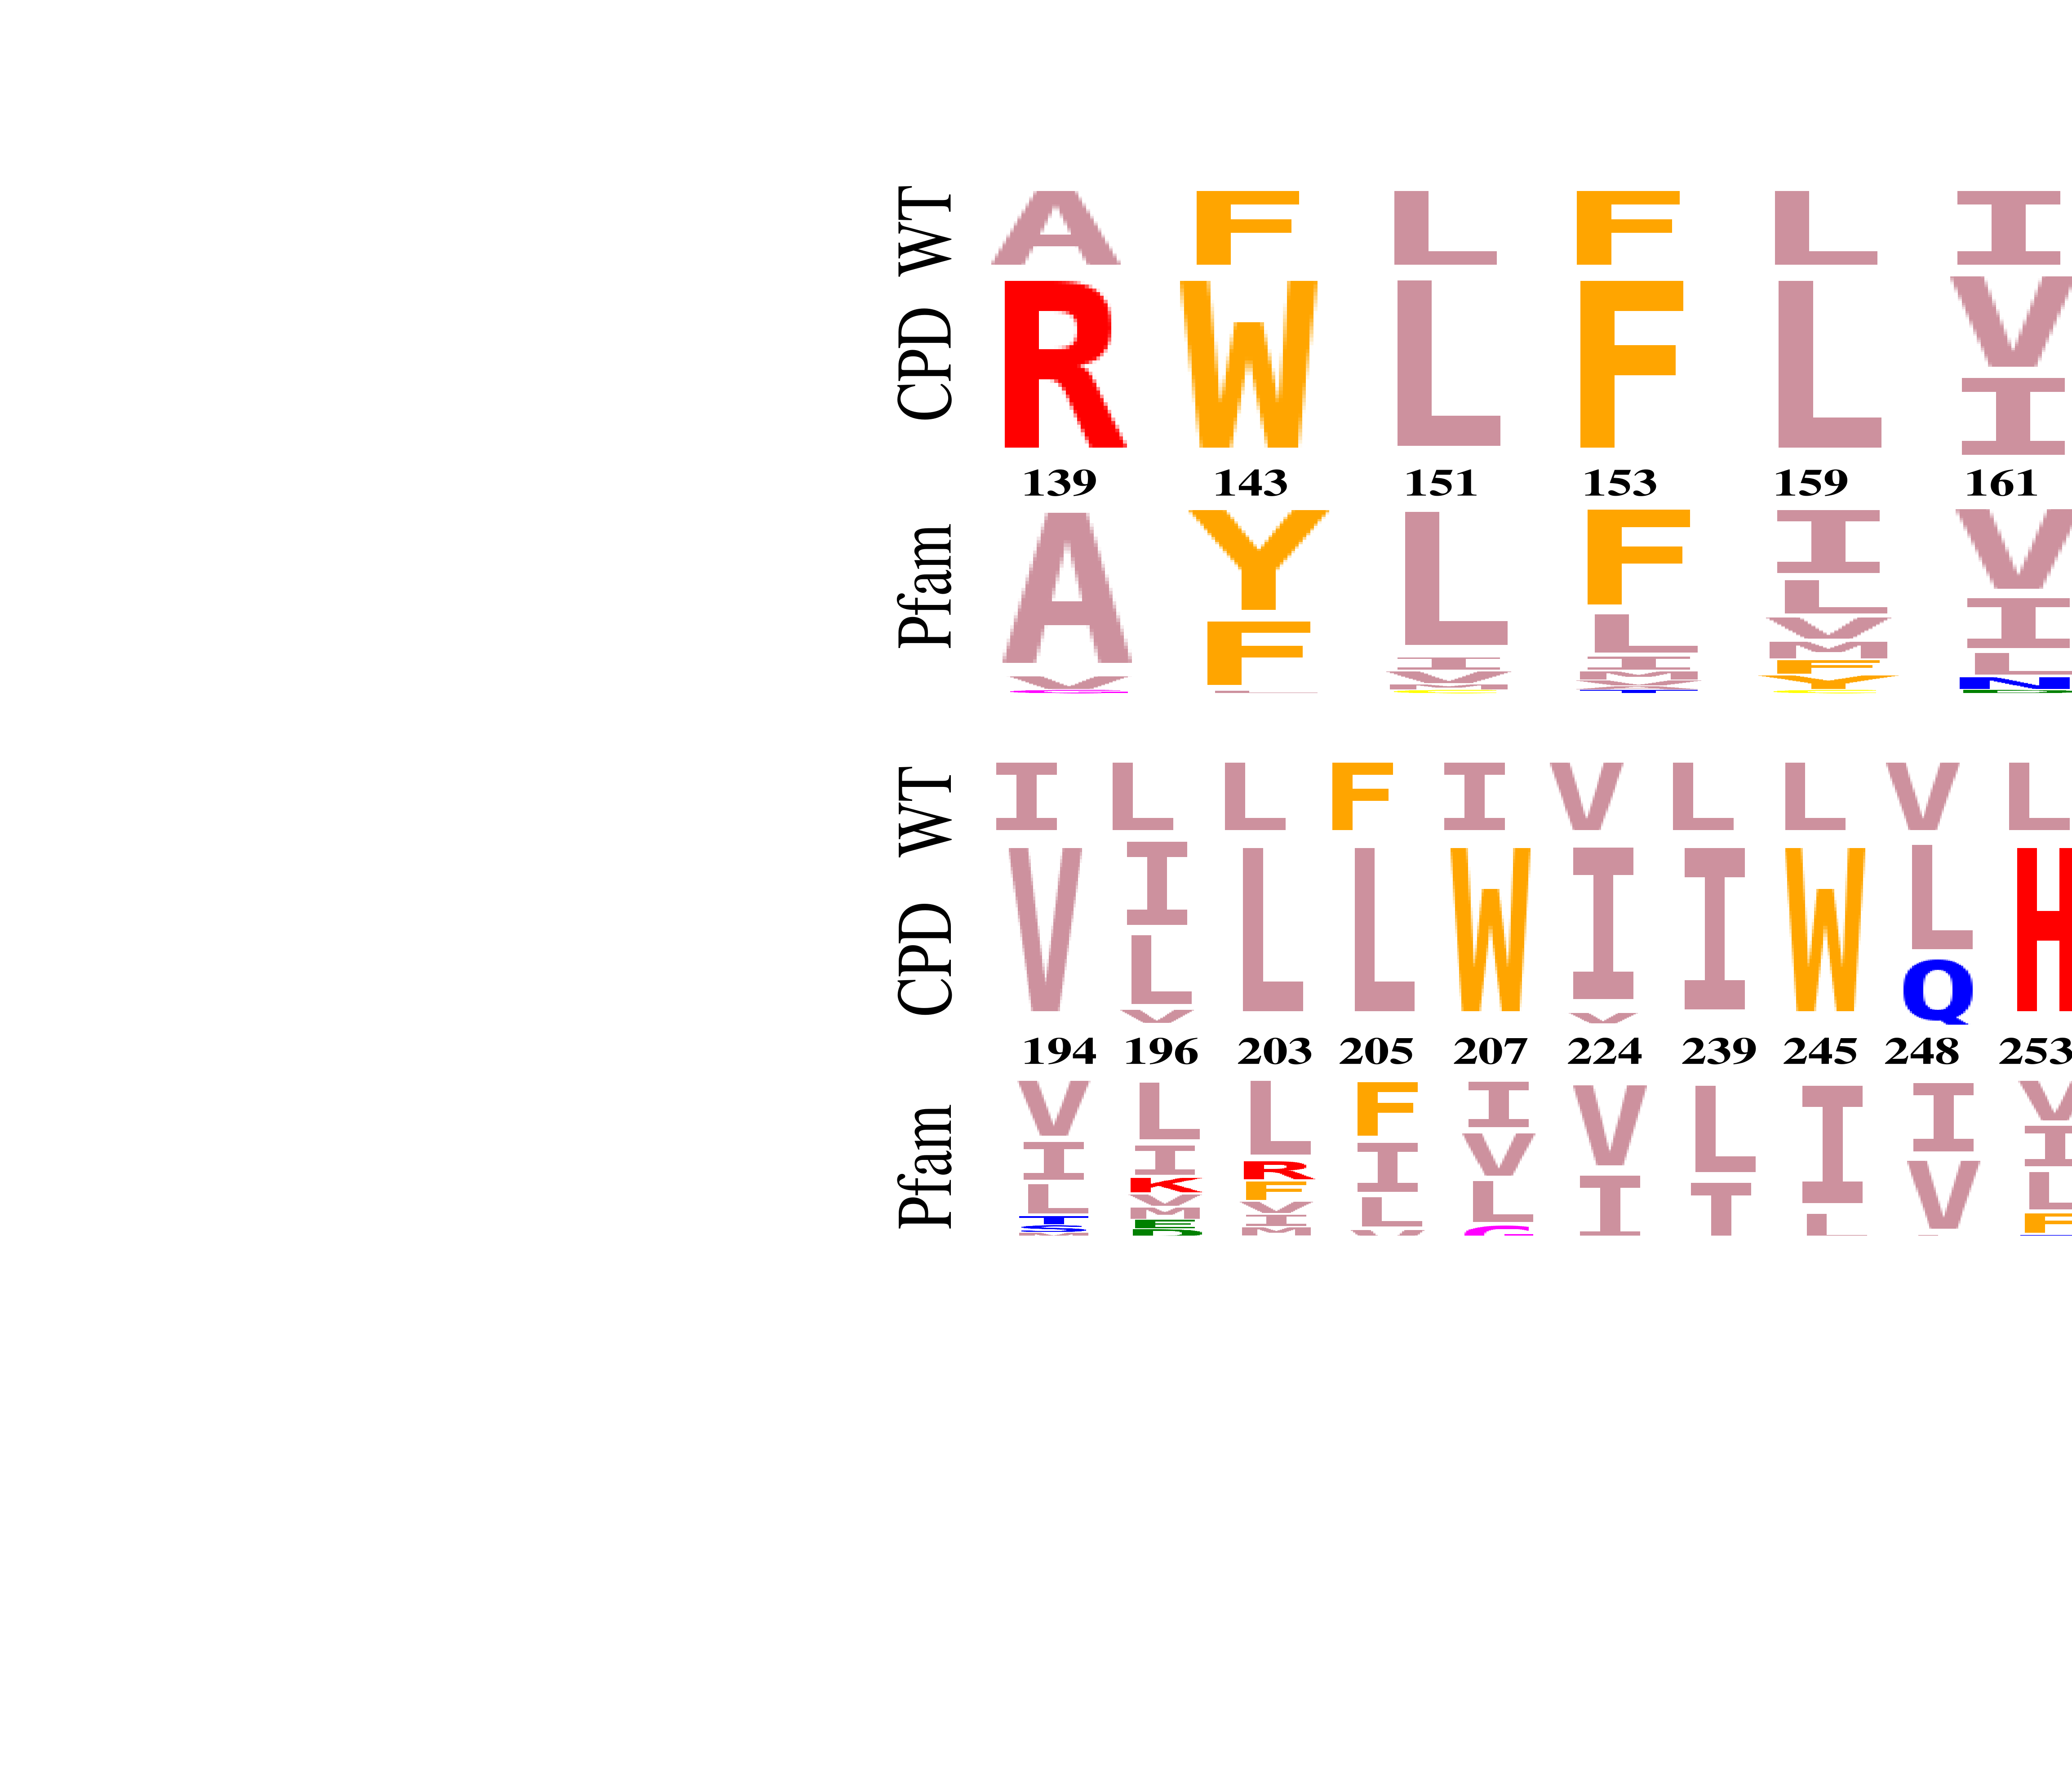
\includegraphics[width=14cm]{align0.png} 
  \caption{
Sequence logos for the core region of two designed proteins: 1CKA (SH3) and 2BYG (PDZ). The low energy CPD sequences are compared to the sequences of the full Pfam collection of
experimental sequences. Positions shown correspond to the hydrophobic core of each protein; residue numbers are indicated (PDB numbering).
}
      \label{fig:logos}
\end{figure}

REMC was done with height replicas at temperatures between 0.175 and 3 $kT$ units. Simulation lengths were 750 million steps (per replica). The top 10000 sequence/conformation combinations were retained, corresponding to 200--400 unique sequences. For eight of the nine test proteins, all the retained sequences were recognized as members of the correct superfamily and family, with match lengths and E-values given in table \ref{tab:quality}. Thus, our designed sequences are mostly similar to experimental ones. Sequence identities to wildtype are 31\% on average (table \ref{tab:quality}), similar to earlier studies with the same energy function \cite{Schmidt09,Schmidt10}. The good agreement with experiment is also illustrated by computing similarity scores between the designed sequences and sequences from the Pfam database. For the protein core region, the similarity is similar to that between experimental sequences, as shown in figure \ref{fig:logos}. Notice that we use here a simple CASA solvent model, since our focus is not the quality of the designed sequences, but the performance of our search algorithms. With a more sophisticated Generalized Born solvent model and a more highly optimized unfolded state model, sequence quality would be even better (manuscript in preparation).

Representative sequence logos for the protein core are shown in Fig.\ \ref{fig:logos}, illustrating the agreement between designed and experimental sequences. For the SH3 protein 1CKA, the design mostly recovers the native sidechain type, or a homologous type that is common in other natural sequences from Pfam. Exceptions include position 170, where we obtain I or V, whereas the native type is W; however, L and V are also occasionally found in Pfam. At position 139, we sample R instead of the native A or V, found in Pfam; however, the hydrophobic part of the designed Arg sidechain is homologous to A and V, while its ionized tip actually sits outside the hydrophobic core, at the protein surface. Finally, at position 143, we sample W, which is homologous to Y and F found in Pfam. For the PDZ domain 2BYG, agreement with the native and Pfam sequences is similar, with a few departures: at positions 207 and 245, we sample W instead of the natural types I, L, V, P; at position 253, we sample H, compared to mostly I, L, V, and sometimes F in Pfam; at position 265,we always sample Y, whereas the Pfam types are diverse (and mostly hydrophobic).

    \begin{figure}[!htbp]
      \centering
      \begin{tabular}{c}
        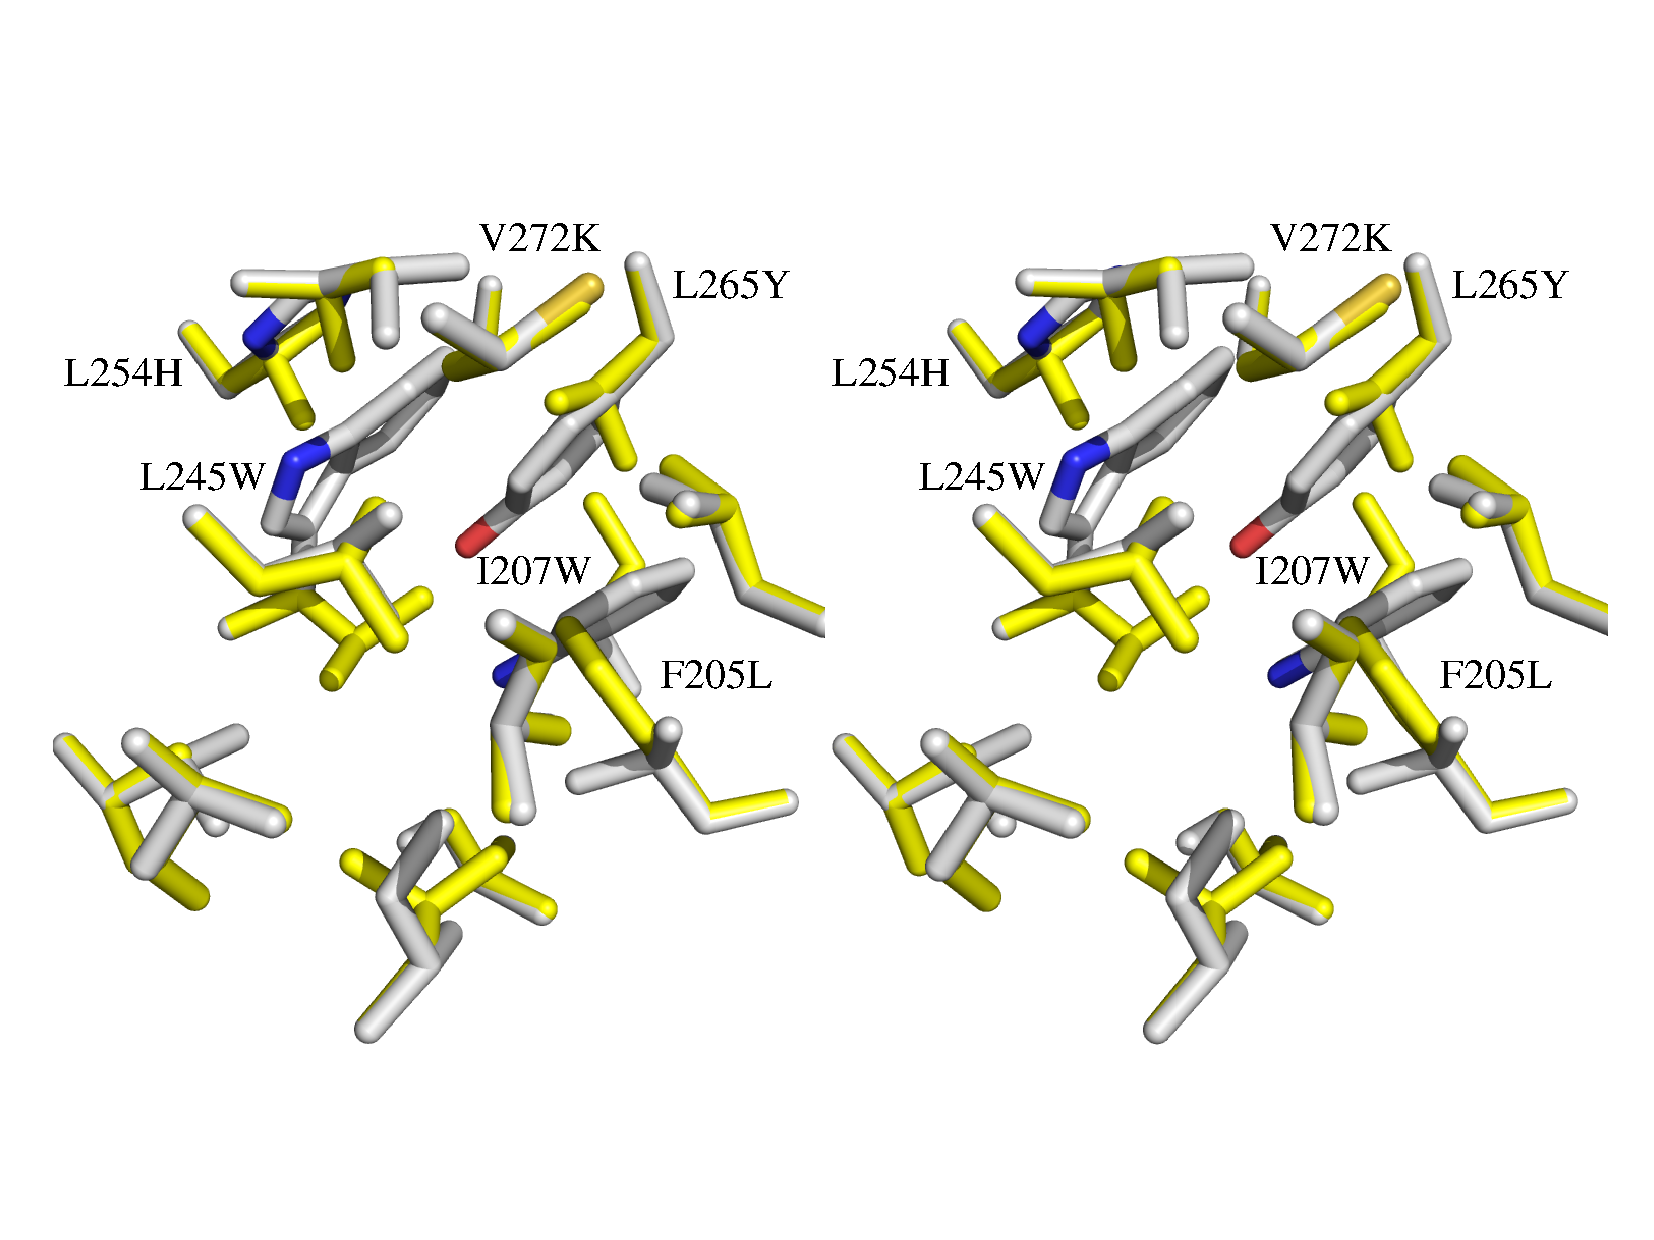
\includegraphics[trim = 0mm 32mm 0mm 10mm, clip, width=12cm]{2BYG_bestall_core3D.pdf} 
      \end{tabular}      
      \caption{The lowest energy sequence/structure combination is shown for the 2BYG PDZ domain (stereo view; selected sidechains only; white sticks), superimposed on the Xray structure (yellow sticks); the sidechains shown are the ones in the sequence logo, Fig.2. The main mutated positions are labelled; other positions are either not mutated or mutated within the ILV group. Figure produced with pymol [72]}
      \label{fig:3Dstruct}
    \end{figure}
For the same PDZ domain, the lowest energy sequence/structure combination is shown in figure \ref{fig:3Dstruct}, superimposed on the Xray structure; only the hydrophobic core sidechains are shown, for clarity. Most of the native/designed sidechains overlap very well, although the double mutation (F205L, L245W) leads to some local repacking.

    For the 1A81 SH2 domain, the lowest energy sequences are not recognized by Superfamily, but if we assay sequences that are 8-12 kcal/mol above the GMEC, about 10\% are correctly recognized by Superfamily as SH3 sequences. Similarly, if the top 10,000 sequences produced by the heuristic algorithm are tested, 57\% of them are recognized by Superfamily as SH3 family members. The heuristic sequences are also 8-12 kcal/mol above the GMEC (see below). This protein illustrates the imperfect parameterization of our energy function, with the consequence that higher energy sequences can actually be more realistic, in some cases, than lower energy ones. Thus, the signifiance of the GMEC is only as good as the energy function.


    \begin{figure}[!htbp]
      \centering
      \begin{tabular}{cc}
        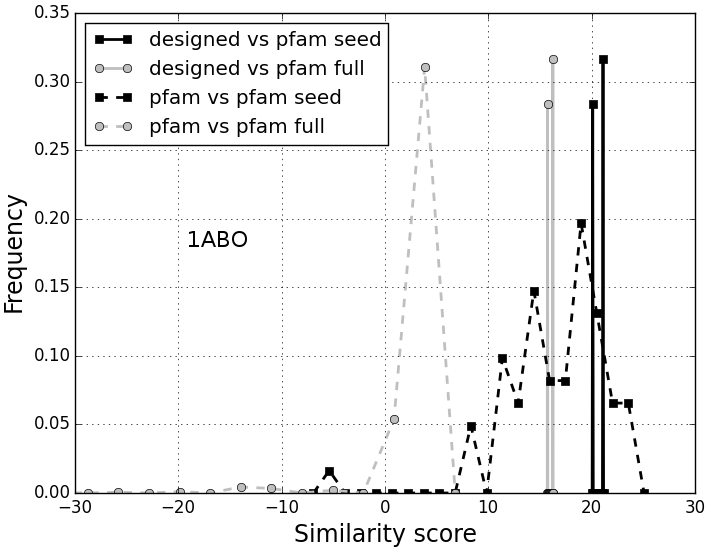
\includegraphics[width=8cm]{1ABO_core_simil_byseq.png} &
        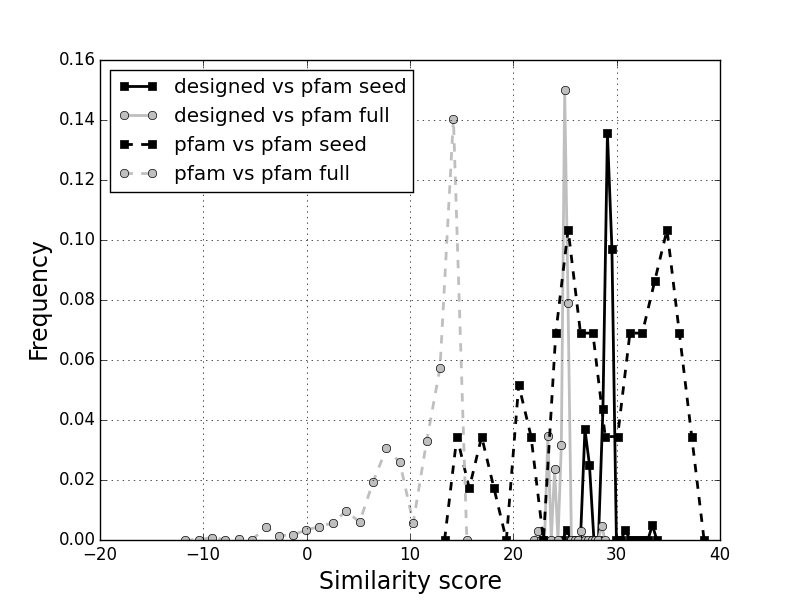
\includegraphics[width=8cm]{1BM2_core_simil_byseq.png} \\
      \end{tabular}
      \caption{Histogram of Blosum40 similarity scores to Pfam sequences for the core region of two
designed proteins: 1ABO (SH3) and 1BM2 (SH2). The similarity between Pfam sequences is
also shown, considering either the Pfam seed alignment or the much larger full alignment.
}
      \label{fig:similarity}
    \end{figure}





\begin{table}[!htbp]                            
\caption{Designed sequence quality measures}
\small
\label{tab:quality}                      
\begin{center}
\begin{tabular}{cccccccc} \hline \hline  
        & Number of & Identity & \multicolumn{5}{c}{\hrulefill Superfamily tests \hrulefill}   \\
        & sequences & \% to    & Match & Superfamily & Superfamily  & Family  & Family        \\
Protein & tested    & wildtype & length & E-value     & success rate & E-value & success rate  \\ \hline
1A81    & 236       & 27       & none   &             &              &         &               \\
1ABO    & 203       & 32       & 51/58  & 4.4e-4      & 100\%        & 2.8e-3  & 100\%         \\
1BM2    & 209       & 27       & 78/98  & 4.2e-5      & 100\%        & 2.6e-3  & 100\%         \\
1CKA    & 416       & 33       & 40/57  & 1.1e-5      & 100\%        & 3.4e-3  & 100\%         \\
1G9O    & 338       & 36       & 79/91  & 7.0e-7      & 100\%        & 2.5e-3  & 100\%         \\
1M61    & 405       & 42       & 97/109 & 7.2e-7      & 100\%        & 2.6e-4  & 100\%         \\
1O4C    & 274       & 21       & 95/104 & 2.1e-4      & 100\%        & 4.5e-3  & 100\%         \\
1R6J    & 270       & 34       & 74/82  & 9.8e-6      & 100\%        & 4.6e-3  & 100\%         \\
2BYG    & 426       & 28       & 59/97  & 1.4e-5      & 100\%        & 7.1e-3  & 100\%         \\ \hline
\end{tabular}
\end{center}
\end{table}



\subsection{Finding the GMEC}
\subsubsection{CPU and memory limits for each method}
\label{BESTprotocol}
The ability of an exploration method to sample low energy sequences depends on the CPU and memory ressources available, as well as on detailed parameterization choices. Here, we set somewhat arbitrary limits, to remain within a practical run situation. For CFN, we set a maximum time limit of 24 h and a memory limit of 30 gbytes (gb). For the heuristic method, we used 110,000 heuristic cycles, increased to 330,000 or 990,000 cycles in a few cases; even for these cases, run times did not exceed 24 h. For MC, we ran up to 10$^9$ simulation steps, which corresponded to CPU times of 9 h at most. For REMC, we ran 0.75 10$^9$ simulation steps per replica, with a few exceptions. We used an OpenMP, shared memory parallelization on a single processor, with one replica per core. Total CPU time per core was never more than 3 hours, for a total CPU use of less than 24 h. For the heuristic, MC, and REMC methods, memory requirements are modest; about 2 gb for the largest calculations. Run times are shown in Fig.\ \ref{fig:cpu} as a function of the number of designed positions, which varies from one position to the entire protein (about 90 positions). For comparison, the CPU time needed to compute the energy matrix for a single pair of designed positions, using an advanced energy function (Generalized Born solvent plus a sophisticated surface area term) and a single core of a recent Intel processor is about 5 hours.


    \begin{figure}[!htbp]
      \centering
        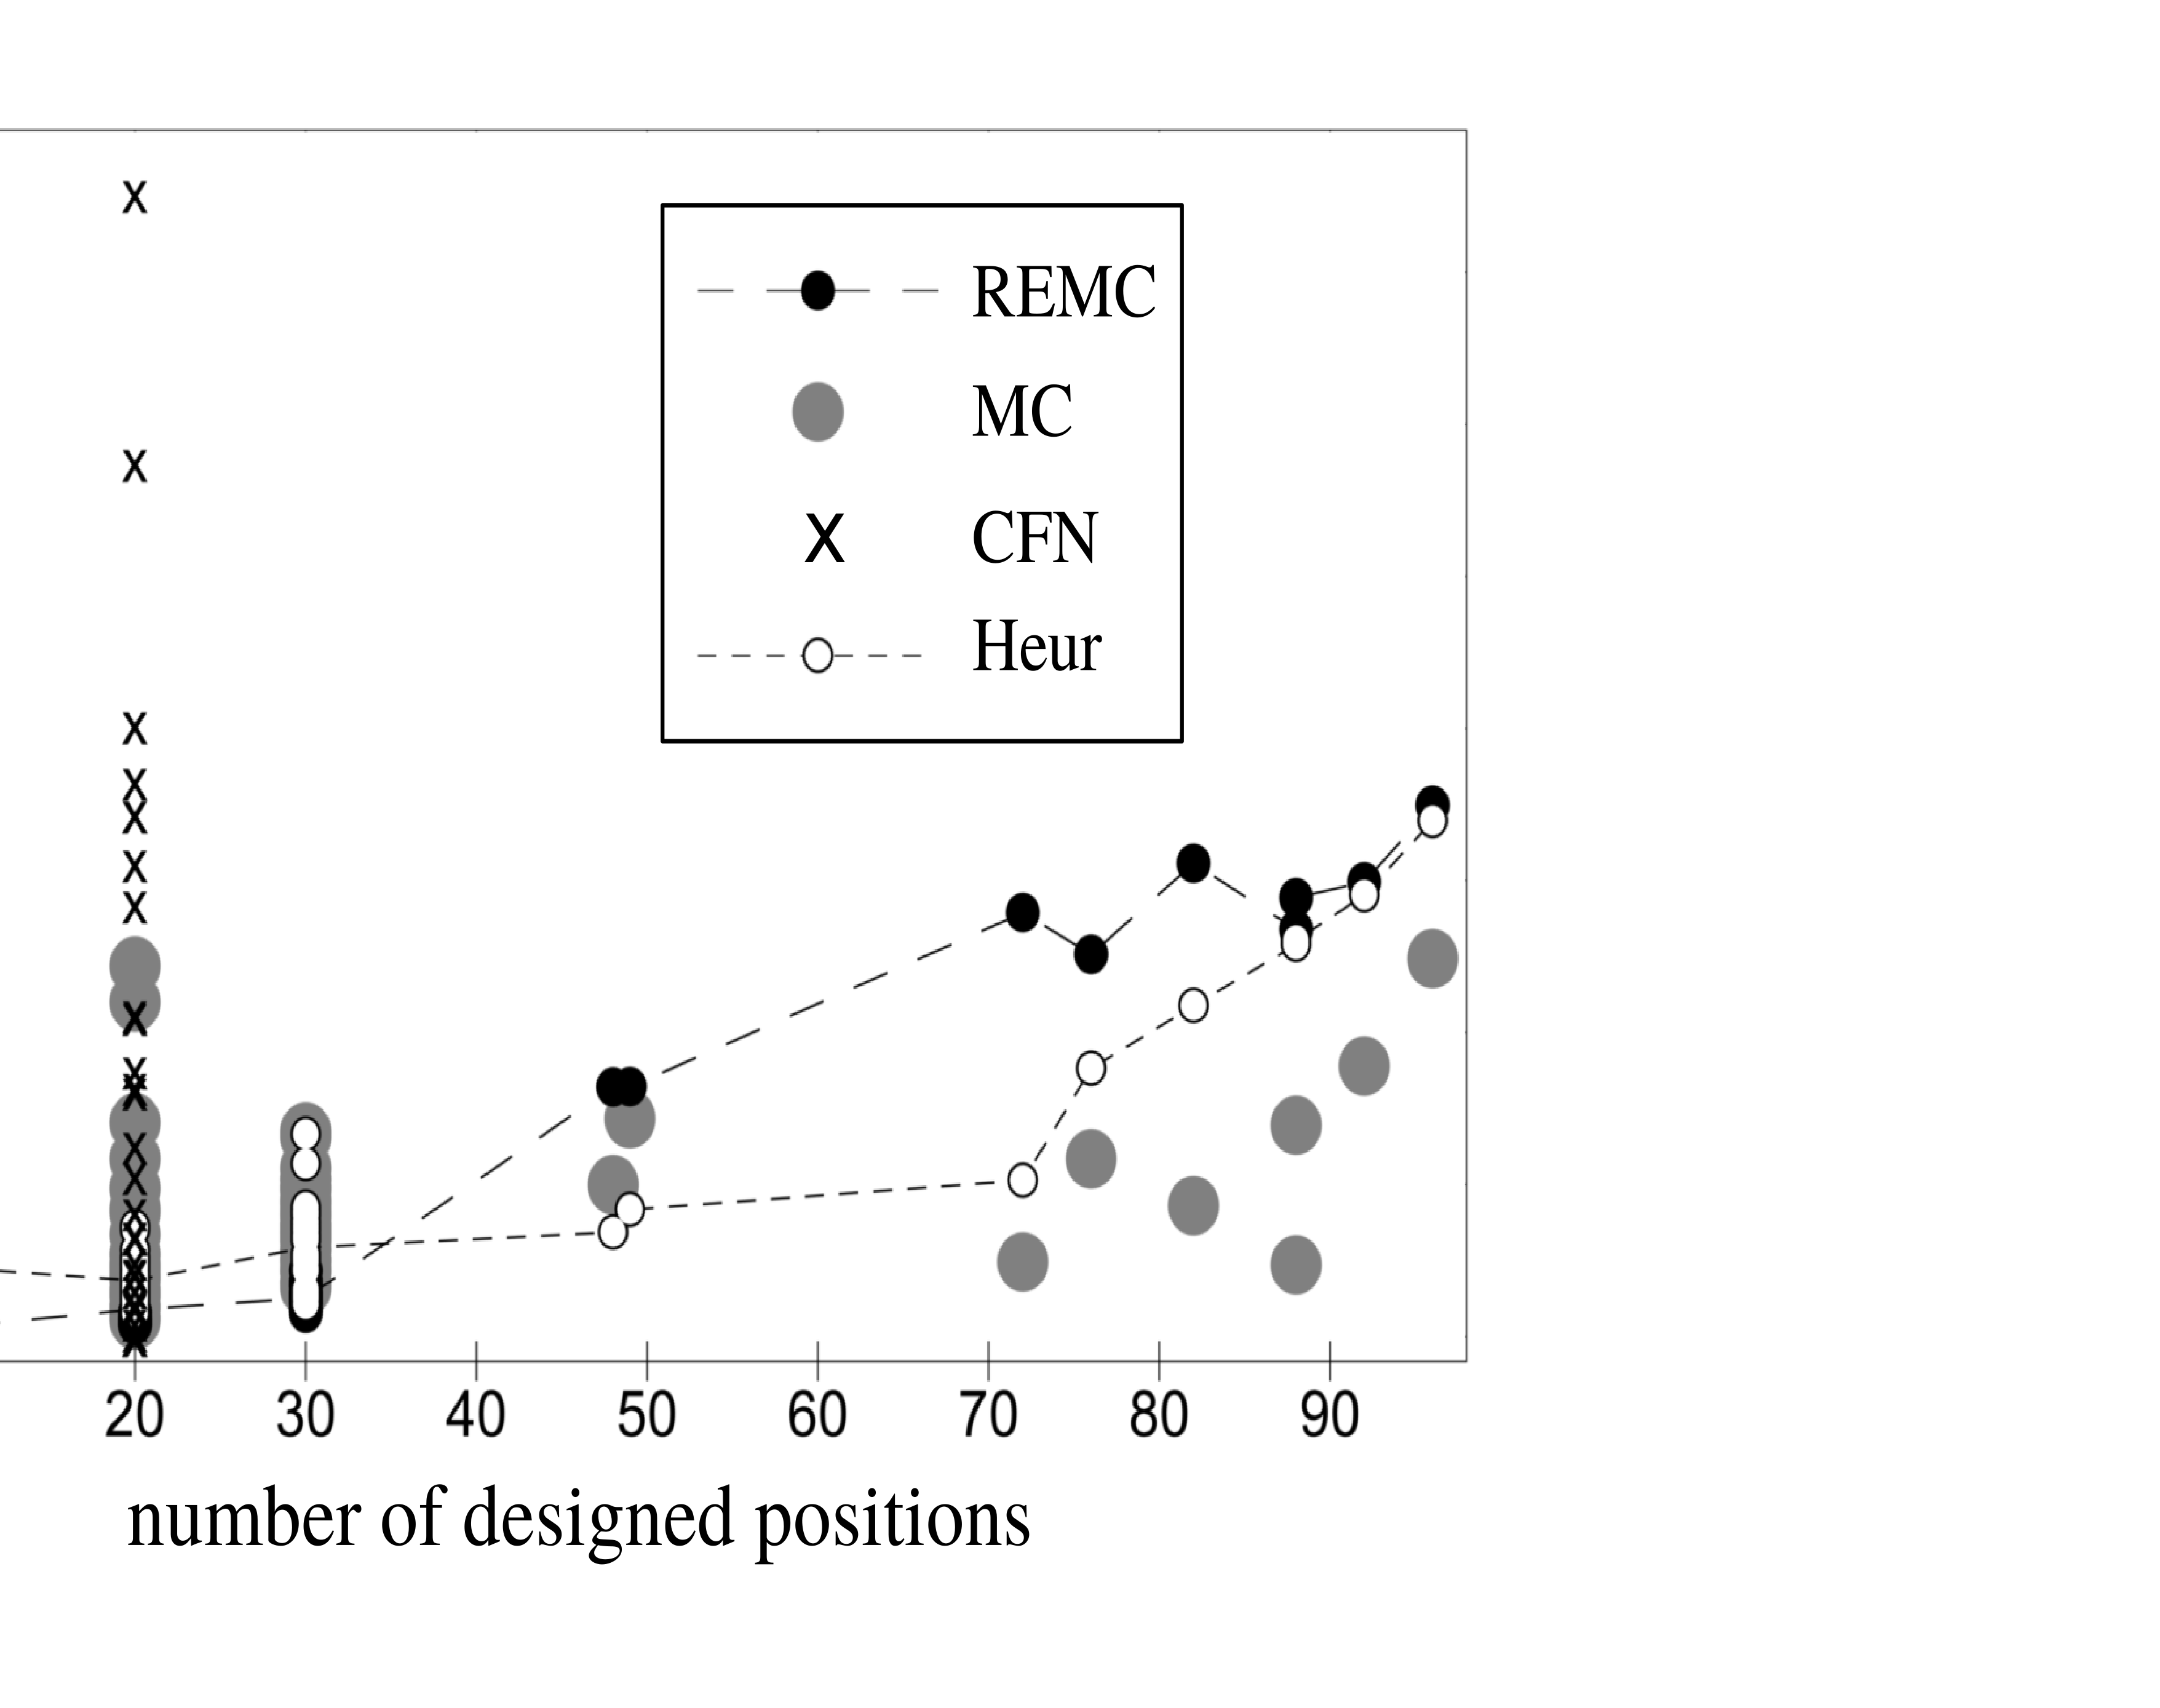
\includegraphics[width=10cm]{speed.png} 
      \caption{
Run times for different test calculations and search methods. CPU times per core are shown; only the REMC calculations use multiple cores (OpenMP parallelization). CFN results are only given for 20 designed positions or fewer. REMC was only done for the larger calculations. Results are shown for a large, representative subset of the test calculations. A few CFN calculations were allowed to run beyond the 24h CPU limit. For clarity, the average Heur and REMC values are included as dashed lines.
      }
      
      \label{fig:cpu}
    \end{figure}

The MC and REMC methods require choices of move probabilities and temperatures, which affect the sampling in ways that vary from protein to protein. Fig.\ \ref{fig:fulldelta} shows the lowest energy sampled with a small collection of protocols: one heuristic, one MC, and five REMC protocols, applied to our nine proteins, with all positions allowed to mutate (except Gly/Pro). The protocol details are given in table \ref{tab:parameters}. For these large design problems, the GMEC is not known. Instead, for each protein, the overall best energy (the best of the seven protocols) is taken as the reference, or zero value.


    \begin{figure}[!htbp]
      \centering
        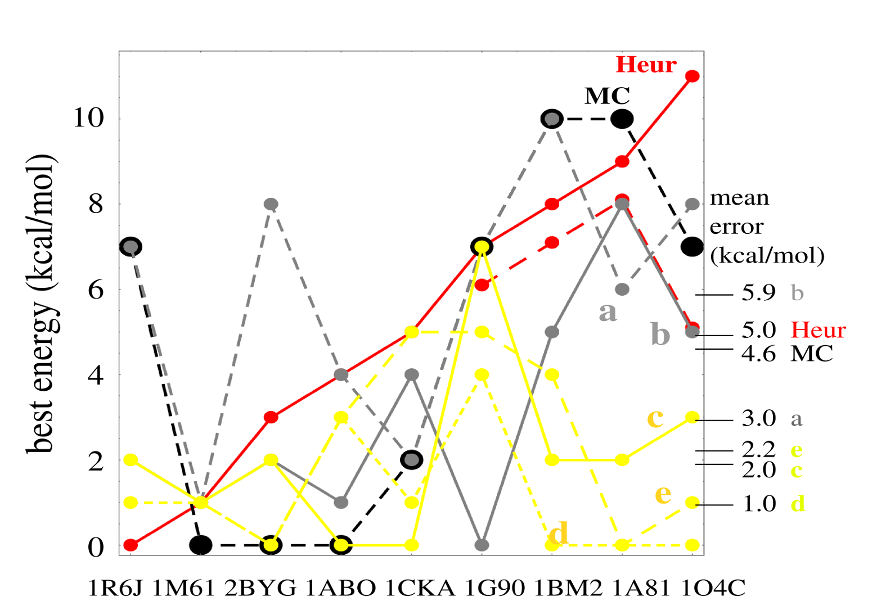
\includegraphics[width=12cm]{full_delta.png} 
      \caption{
Comparison between selected heuristic, MC, and REMC protocols for whole protein design. The best energy obtained with each protocol is shown for the nine test proteins. Zero represents the overall best energy for each protein. The mean ``error'' is indicated on the right for each protocol (the mean difference from the overall best energy). The protocols are a heuristic method (Heur), an MC method, two REMC protocols with 4 walkers (REMC a, b), and three REMC protocols with 8 walkers (yellow lines and dots, REMC c, d, e). Details of the protocols are in table \ref{tab:parameters}; each curve is labelled according to the protocol name.
}
       \label{fig:fulldelta}
    \end{figure}

For a given protein, the best energy varies by up to 12 kcal/mol from one protocol to another (compare the 1BM2 REMCa and REMCc energies or the 1CKA MC and REMCd energies). For each protocol, the best energy obtained was averaged over the nine proteins, giving a mean ``error''; these values are also reported in Fig.\ \ref{fig:fulldelta}. The lowest mean error is 1.0 kcal/mol, with REMCd. In other words, REMCd gives a best energy that is, on average, 1.0 kcal/mol above the overall best energy. Based on these and other similar tests, for the rest of this work, we used the specific MC protocol in table \ref{tab:parameters} and the REMCd replica exchange protocol, which are generally good but not necessarily optimal for every situation. 

\subsubsection{Optimal sequences/structures with up to 10 designed positions}
As our first series of tests, we did calculations for each test protein with zero, one, or five designed positions. Results are summarized in Fig.\ \ref{fig:fulldelta}. With zero positions, only rotamers are optimized (at all positions in the protein). With one, we systematically designed each position of each protein in turn (plus rotamers at all positions). With 5, we picked the positions randomly, close together in the structure, in five different ways, for a total of 45 tests. Two positions were considered close by if they have at least one rotamer combination that gives an interaction energy of 10 kcal/mol or more (in absolute magnitude; eg, steric overlap). In all these cases, CFN found the GMEC very rapidly (seconds); the heuristic also found the GMEC, with much longer run times (an hour). MC found the GMEC in all but a few cases (Fig.\ \ref{fig:errors}), with run times of a few minutes. 

\begin{figure}[!htbp]
  \begin{center}
    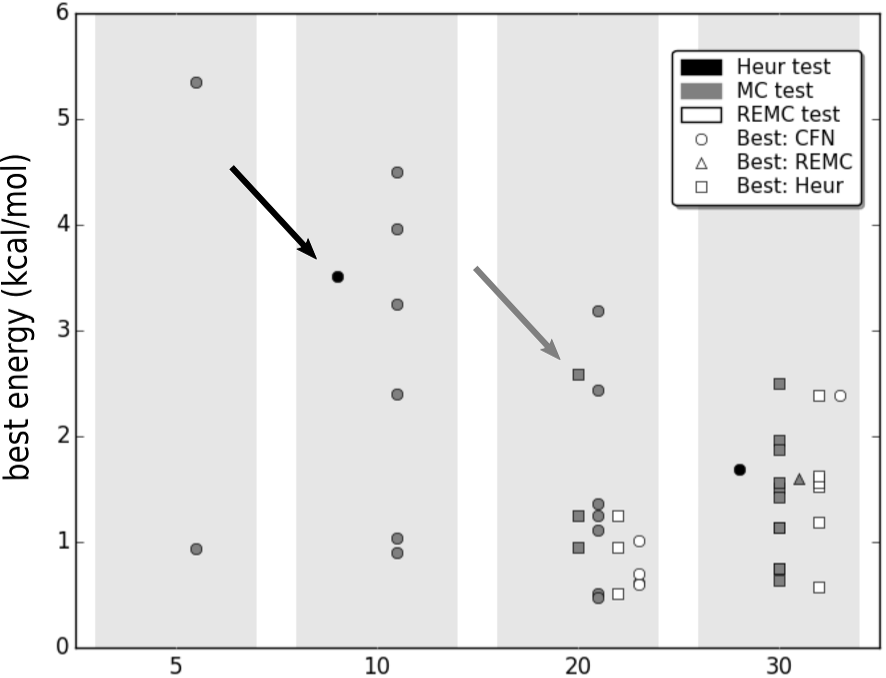
\includegraphics[width=10cm]{errors.png}
  \end{center}
  \caption{The lowest energies obtained with the different exploration
methods for 5-, 10-, 20-, and 30-position design. Differences with respect
to the GMEC or the overall best energy are shown, excluding the smallest
values (less than 0.4 kcal/mol above the best energy). The color of each
point indicates the nature of the test; its shape indicates which method
gave the best energy. Two examples are highlighted by arrows: the black
arrow shows the heuristic result for a 10-position test where the best
energy was given by CFN; the gray arrow shows the MC result for a 20-
position test where the best energy was given by the heuristic. The dashed
red line shows heuristic results with a more aggressive protocol (330,000
heuristic cycles) for the four rightmost proteins.
}
      \label{fig:errors}
\end{figure}

As a second series of tests, we chose randomly for each protein a set of 10 positions to design; the other positions had fixed types but explored all possible rotamers. The selected positions were close by in the protein structure. For each protein, we made five separate choices of positions to design, for a total of 45 test cases. The CFN, heuristic, and MC methods were run for all 45 cases; REMC was run only when MC gave a poor result (6 cases, involving 5 proteins).
Results are summarized in Fig.\ \ref{fig:errors} and table \ref{tab:10act}. Twenty cases where all methods found the GMEC are not listed in the table, leaving 25 where at least one method did not find the GMEC. CFN performed very well: only in one case did it not find the GMEC. The lowest energy was sampled in this case with the heuristic, and the best CFN energy was 5.7 kcal/mol higher (despite using the more aggressive CFN protocol). With a third, more recent CFN protocol \cite{Simoncini15}, this result did not change. 

The heuristic performed about as well as CFN for 10-position design. In one case, CFN did not find the GMEC and the heuristic gave the lowest energy (2BYG-1). In 39 cases, the heuristic found the GMEC. In three cases, it was within 0.15 kcal/mol of the GMEC, with no mutations (only rotamer differences). In one case (1CKA-5), it was 0.29 kcal/mol above the GMEC, with no mutations. Tripling the number of heuristic cycles allowed the GMEC to be reached (within 0.07 kcal/mol) in all these cases, with run times below 6 h. There was only one real failure, 1M61-2, where the best heuristic solution was 3.5 kcal/mol above the GMEC, with three mutations relative to the GMEC. For this case, the GMEC was recovered (within 0.01 kcal/mol) if the number of cycles was increased to 990,000, for a run time of 7 h. Switching from the heuristic structure (after 330,000 cycles) to the GMEC requires concerted changes in 3 adjacent sidechain positions. This is only possible during a heuristic cycle if there is a downhill, connecting pathway made of single position changes, which is evidently very rare for this particular test. Thus, the heuristic method can only find the GMEC if it draws the right combination of types/rotamers at the very beginning of a cycle; hence the need for 990,000 cycles.

\begin{table}[!htbp]                            
\caption{Tests with 10 designed positions}
\small \label{tab:10act}               
\begin{center}
\begin{tabular}{cccccccc} \hline \hline  
rotamers$^a$& length$^b$& Protein& CFN$^c$ & Heur.$^d$ &  MC & REMC \\ \hline
2991  & 108(17) & 1A81 3 & gmec& 0.001  &  0.1595   &         \\         
      &         & 1A81 4 & gmec& 0.     &  0.0317   &         \\    
      &         & 1A81 5 & gmec& 0.     &  0.0563   &         \\    
2520  & 58(8)   & 1ABO 1 & gmec& 0.0675 &  0.9054   & 0.8041  \\   
      &         & 1ABO 4 & gmec& 0.     &  0.0128   &         \\            
2957  & 98(10)  & 1BM2 1 & gmec& 0.     &  0.0950   &         \\         
      &         & 1BM2 5 & gmec& 0.     &  0.1082   &         \\    
2508  & 57(8)   & 1CKA 5 & gmec& 0.2859 &  3.2525   & 0.      \\           
2819  & 91(15)  & 1G9O 3 & gmec& 0.1366 &  0.1366   &         \\ 
      &         & 1G9O 5 & gmec& 0.     &  3.9599   & 0.      \\ 
2957  & 109(21) & 1M61 1 & gmec& 0.     &  0.0776   &         \\               
      &         & 1M61 2 & gmec& 3.5105 &  4.5062   & 0.3215  \\               
      &         & 1M61 5 & gmec& 0.     &  0.0432   &         \\     
3037  & 104(8)  & 1O4C 1 & gmec& 0.     &  0.1121   &         \\    
      &         & 1O4C 2 & gmec& 0.     &  0.1046   &         \\         
      &         & 1O4C 3 & gmec& 0.     &  0.1519   &         \\             
      &         & 1O4C 4 & gmec& 0.     &  0.1545   &         \\             
      &         & 1O4C 5 & gmec& 0.     &  0.1753   &         \\      
2773  & 82(10)  & 1R6J 1 & gmec& 0.     &  2.4022   & 0.3986  \\        
      &         & 1R6J 2 & gmec& 0.     &  1.0398   & 0.3049  \\        
      &         & 1R6J 3 & gmec& 0.     &  0.0106   &         \\       
      &         & 1R6J 5 & gmec& 0.     &  0.0162   &         \\        
2888  & 97(15)  & 2BYG 1 & 5.7485& 0.   &  0.0337   &         \\        
      &         & 2BYG 3 & gmec& 0.     &  0.0833   &         \\        
      &         & 2BYG 4 & gmec& 0.     &  0.2149   &         \\        
\hline
\end{tabular}
\end{center}
{\small \noindent $^a$Total number of rotamers available to the system. 
Each designed position can explore 206 rotamers; the others explore about 10 rotamers each. $^b$Total protein length (number of Gly+Pro in parentheses).
$^c$gmec indicates the GMEC was successfully identified. $^d$For all four exploration methods and each test, we report the difference between the best energy obtained and the overall best energy (the best over all methods, which may or not be the GMEC). 10-position tests where all four methods found the GMEC are not listed.
}
\end{table}



Plain MC did slightly less well for 10-position design. In 21 cases, it found the GMEC. In 18 cases, its best sequence was within 0.2 kcal/mol of the GMEC, with 0--3 mutations (one on average). Notice that 0.2 kcal/mol is the thermal energy for the MC protocol used. In six cases, its best sequence was between 0.9 and 4.5 kcal/mol above the GMEC, with 2--7 mutations (3 on average). For these six cases, REMC was run, and sampled sequences within 0.40 kcal/mol of the GMEC, except for one case where its best sequence was 0.80 kcal/mol above the GMEC. Overall, MC or REMC reached the GMEC to within 0.40 kcal/mol in all but one case. A 0.40 kcal/mol energy difference is actually less than the average pairwise additivity errors in the energy function \cite{Lopes07,Schmidt08b,Gaillard14}, and so one might consider this performance to be about as good as the CFN and heuristic methods. In terms of speed, for 10-position design, all the methods were comparable (a few hours per run on average).

\subsubsection{Optimal sequences with 20 or 30 designed positions}
We did similar tests with 20 designed positions, selected randomly in 5 different ways for each protein, as above.
Results are given in Fig.\ \ref{fig:errors} and table \ref{tab:20act}. CFN found the GMEC in 28 out of 45 cases;
in two others, it found the best energy of the four methods. For 6 of these 30 cases, the more aggressive protocol was necessary, and run times were 2--22 h (11 on average). For 14 of the other 15 cases, the best CFN energy was 0.1--7.5 kcal/mol above the best solution found by the other methods, and 2.8 kcal/mol on average, despite using the more aggressive protocol. For the worst case, the CFN energy was 13.9 kcal/mol above the best solution. Of th 17 cases where the CFN was not identified, half were rerun with a third, more recent CFN protocol \cite{Simoncini15}; in just one of these cases (1BM2-4, a very mild failure) did the newer protocol identify the GMEC.

The heuristic method found the GMEC in 22 of the 28 cases where it is known. For the other six cases, it was within 0.40 kcal/mol of the GMEC, with 0--4 mutations (2.7 on average). For the 17 cases where the GMEC was not identified by CFN, the heuristic produced the lowest energy of all methods, except one case (104C-1) where it was 0.35 kcal/mol above CFN.
Overall, the heuristic either found the best energy of the four methods or was within 0.40 kcal/mol of the best energy.

MC converged to the best energy in 11 cases; in 25 other cases, it was within 0.50 kcal/mol of the best energy. In the other nine cases, its best energy was at most 3.2 kcal/mol above the best energy (sampled by the heuristic and/or CFN).
Finally, REMC was done for all the test cases. In six cases, its best energy was more than 0.50 kcal/mol from the best energy. However, the differences were notably smaller than for plain MC, with an average of just 0.8 kcal/mol for the 6 worst cases and a maximum (for 1G90-1) of 1.25 kcal/mol.

The same tests were done with 30 designed positions; see Fig.\ \ref{fig:errors} and table \ref{tab:20act}. CFN found the GMEC in just one case; in 5 others, it did not find the GMEC but gave the lowest energy overall. In four other cases, it was within 0.50 kcal/mol of the best energy sampled by the other methods. For the other 35 cases, its best energy was higher than the best method, with differences of 10 kcal/mol or more in 20 cases.


\begin{table}[!htbp]   
%\vspace*{-2.5cm}                         
\caption{Tests with 20 and 30 designed positions}
\footnotesize \label{tab:20act}               
\begin{center}
\begin{tabular}{cccccccccc} \hline \hline  
       & \multicolumn{5}{c}{\hrulefill~20 positions~\hrulefill} & \multicolumn{4}{c}{\hrulefill~30 positions~\hrulefill} \\
Protein&  CFN     & Heur.\ & MC     & REMC   & mutations$^a$ & CFN & Heur.\ & MC & REMC \\ \hline
1A81 1 &  gmec*   & 0.     & 0.3275 & 0.3851 & 0 & 1.2074    & 0.     & 0.6353 &        \\         
1A81 2 &  gmec*   & 0.1705 & 2.4355 & 1.0069 & 3 & 2.5520    & 0.     & 0.0578 &        \\   
1A81 3 &  gmec    & 0.     & 0.4640 & 0.6186 & 0 & 43.5263   & 0.     & 2.4996 & 1.2025 \\         
1A81 4 &  gmec    & 0.3878 & 0.5748 & 0.6991 & 4 & 5.1300    & 0.     & 0.0305 &        \\    
1A81 5 &  gmec    & 0.0068 & 0.5088 & 0.1541 & 4 & 3.2417    & 0.     & 1.9586 & 0.5791 \\    
1ABO 1 &  gmec    & 0.1205 & 1.1159 & 0.2153 & 2 & 44.5504   & 0.     & 0.     &        \\   
1ABO 2 &  13.8563 & 0.     & 0.     & 0.     & 8 & 12.7303   & 0.     & 0.     &        \\               
1ABO 3 &  1.2190  & 0.     & 0.     & 0.     & 9 & 9.3870    & 0.     & 0.2630 &        \\                 
1ABO 4 &  1.9940  & 0.     & 0.0076 & 0.     & 5 & 10.7691   & 0.     & 0.     &        \\            
1ABO 5 &  3.5418  & 0.     & 0.9483 & 0.9483 & 9 & 4.3907    & 0.     & 0.     &        \\       
1BM2 1 &  gmec    & 0.     & 0.0619 & 0.1584 & 0 & 22.5876   & 0.     & 1.7290 & 1.6013 \\         
1BM2 2 &  7.5304  & 0.     & 0.0725 & 0.0143 & 8 & 22.1386   & 0.     & 1.9856 & 1.5876 \\     
1BM2 3 &  gmec    & 0.0229 & 0.4762 & 0.2897 & 0 & 22.5410   & 0.     & 1.9990 & 1.1541 \\    
1BM2 4 &  0.1186  & 0.     & 2.5883 & 0.0789 & 2 & 15.2639   & 0.     & 2.2127 & 2.3854 \\     
1BM2 5 &  gmec    & 0.2396 & 0.3746 & 0.3746 & 3 & 15.9890   & 0.     & 2.8354 & 1.1937 \\    
1CKA 1 &  gmec*   & 0.     & 0.     & 0.     & 0 & 6.2700    & 0.     & 0.     &        \\                   
1CKA 2 &  gmec    & 0.     & 0.     & 0.     & 0 & 2.0995    & 0.     & 0.     &        \\                   
1CKA 3 &  gmec    & 0.     & 0.     & 0.     & 0 & 47.0217   & 0.     & 0.     &        \\                   
1CKA 4 &  4.3122  & 0.     & 0.     & 0.     & 4 & 44.0830   & 0.     & 0.     &        \\               
1CKA 5 &  4.2849  & 0.     & 0.     & 0.     & 3 & 8.8608    & 0.     & 0.     &        \\           
1G9O 1 &  2.0574  & 0.     & 1.2525 & 1.2525 & 5 & 2.0816    & 0.     & 1.5942 & 0.     \\ 
1G9O 2 &  3.2106  & 0.     & 0.2177 & 0.1915 & 1 & 0.3270    & 0.     & 0.3126 &        \\ 
1G9O 3 &  1.9008  & 0.     & 0.4417 & 0.1019 & 1 & 17.7150   & 0.     & 1.5667 & 1.5667 \\ 
1G9O 4 &  0.5030  & 0.     & 0.3855 & 0.1455 & 5 & 2.9758    & 0.     & 1.4284 & 1.6202 \\ 
1G9O 5 &  0.4298  & 0.     & 0.1495 & 0.5114 & 5 & 0.        & 1.6890 & 7.6985 & 2.3857 \\ 
1M61 1 &  gmec    & 0.     & 0.     & 0.     & 0 & 14.4935   & 0.0097 & 0.     & 0.     \\                   
1M61 2 &  gmec    & 0.     & 0.     & 0.     & 0 & 5.0899    & 0.     & 1.8749 & 0.008  \\                   
1M61 3 &  gmec    & 0.     & 0.     & 0.     & 0 & 3.5795    & 0.     & 0.0154 &        \\                   
1M61 4 &  gmec    & 0.     & 0.     & 0.     & 0 & 16.1511   & 0.     & 0.     &        \\                   
1M61 5 &  gmec    & 0.     & 0.2521 & 0.1345 & 0 & 23.0927   & 0.     & 0.     &        \\     
1O4C 1 &  0.      & 0.3465 & 0.0690 & 0.0587 & 6 & 14.9064   & 0.     & 0.3435 &        \\    
1O4C 2 &  6.4214  & 0.     & 0.1963 & 0.3175 & 4 & 58.1558   & 0.     & 0.0795 &        \\         
1O4C 3 &  gmec    & 0.     & 0.3461 & 0.0997 & 0 & 9.9221    & 0.     & 0.1789 &        \\             
1O4C 4 &  gmec    & 0.     & 0.3640 & 0.1382 & 0 & 5.7790    & 0.     & 0.0423 &        \\             
1O4C 5 &  0.      & 0.     & 0.1131 & 0.2206 & 0 & 9.9221    & 0.     & 0.1789 &        \\      
1R6J 1 &  gmec    & 0.     & 0.2604 & 0.2002 & 0 & gmec*     & 0.     & 0.0246 &        \\        
1R6J 2 &  gmec    & 0.     & 0.0071 & 0.0183 & 0 & 14.9800   & 0.     & 0.0957 &        \\        
1R6J 3 &  gmec    & 0.     & 0.0537 & 0.0732 & 0 & 0.        & 0.     & 0.0440 &        \\       
1R6J 4 &  gmec    & 0.     & 0.0639 & 0.0601 & 0 & 0.        & 0.     & 0.0957 &        \\        
1R6J 5 &  gmec    & 0.     & 0.0735 & 0.0244 & 0 & 0.        & 0.7036 & 1.8823 & 0.0781 \\        
2BYG 1 &  gmec    & 0.     & 3.1878 & 0.0257 & 0 & 17.9752   & 0.     & 0.1592 &        \\        
2BYG 2 &  gmec    & 0.     & 0.0524 & 0.0831 & 0 & 0.3832    & 0.     & 0.1502 &        \\        
2BYG 3 &  gmec*   & 0.     & 1.3564 & 0.0826 & 0 & 0.1442    & 0.     & 0.1593 &        \\        
2BYG 4 &  gmec    & 0.     & 0.1968 & 0.6022 & 0 & 0.        & 0.0958 & 0.0050 &        \\        
2BYG 5 &  1.8604  & 0.     & 0.0933 & 0.0386 & 2 & 0.5003    & 0.     & 0.6876 &        \\   
\hline
\end{tabular}
{\small \noindent Format as in table \ref{tab:10act}. gmec* indicates the more aggressive protocol.
$^a$Between CFN/Heur.}
\end{center}
\end{table}




The heuristic produced the lowest energy in all but four cases, with differences in those cases of 0.01, 0.10, 0.70, and 1.69 kcal/mol from the best energy. In the last two cases, CFN produced the best energy. Plain MC found the best energy in only 12 cases, but gave only moderate energy errors: in just four cases was its best sequence more than 2 kcal/mol above the overall best energy (differences of 2.2, 2.5, 2.8, and 7.7 kcal/mol). REMC was applied to the 14 cases where the MC errors were largest; in four of these it reduced the error to 0.6 kcal/mol or less. The largest MC error was reduced from 7.7 to 2.4 kcal/mol. Doubling the REMC trajectory length ( to 1.5 billion steps, 1G9O-5) reduced the largest remaining errors to 1.1 and 1.8 kcal/mol.

\subsection{Density of states above the GMEC}
The exact CFN method can enumerate exhaustively sequence/conformation states above the GMEC, up to a given energy threshold, if the threshold is not too large. MC and REMC explore states randomly, within a typical energy range that depends on temperature. To characterize the diversity of the sequence ensembles, we focus on the CFN and REMC methods, and we consider both the sequence entropy and the total number of states. 

The mean, exponentiated sequence entropies $\langle e^{S_i}\rangle$ are reported in table \ref{tab:entropy} for each test protein. The sequence entropies for the corresponding Pfam alignments (both seed and full) are also shown. The values are averaged over the designed positions in the protein chain, and can be interpreted as a mean number of amino acid classes sampled at each position. There are six classes (see Methods), one of which (Gly) is not available to the designed positions but is present in Pfam. The entropies are much smaller in the designed sets than in the Pfam sets.


\begin{table}[!htbp]                            
\caption{Designed and Pfam sequence entropies}
\label{tab:entropy}                      
\begin{center}
\begin{tabular}{ccccc} \hline \hline  
        & Top 10,000 & Top 10,000 & Pfam & Pfam \\
Protein & structures & sequences  & seed & full \\ \hline
1ABO & 1.36 & 1.58 & 2.79 & 3.01 \\
1CKA & 1.20 & 1.41 & 2.84 & 3.03 \\
1R6J & 1.33 & 1.48 & 3.11 & 3.66 \\
1G9O & 1.21 & 1.53 & 3.29 & 3.81 \\
2BYG & 1.57 & 1.63 & 3.31 & 3.67 \\
1BM2 & 1.08 & 1.26 & 2.90 & 3.50 \\
1O4C & 1.36 & 1.68 & 2.94 & 3.47 \\
1M61 & 1.31 & 1.41 & 2.91 & 3.51 \\
1A81 & 1.13 & 1.29 & 2.91 & 3.51 \\ \hline
\end{tabular}
\end{center}
{\small \noindent The entropies are exponentiated, then averaged over all positions.
The designed entropies correspond to REMC runs where all positions are designed (except Gly/Pro).}
\end{table}


Retaining the top 10,000 designed sequences, CPD samples 1.3 to 1.7 amino acid classes at each position on average, compared to 3--4 in the Pfam alignments, or 2--3 Pfam classes if we exclude the Gly class. Thus the CPD sets are much less diverse than Pfam, as observed earlier for these and other protein families \cite{Schmidt09,Schmidt10}. However, we showed earlier that if we did CPD for around ten backbone conformations, corresponding to ten representatives of a particular domain class (SH3, SH2, PDZ), then collected the sampled sequences, the overall entropy was similar to Pfam \cite{Schmidt09,Schmidt10}. 

The sequence entropy $S(E)$ is shown in figure \ref{fig:entropy} for the 1CKA SH3 protein as a function of the energy threshold $E$. Exact CFN results are compared to REMC. For this small protein, complete enumeration was feasible up to an energy threshold of $E$ = 2 kcal/mol above the GMEC. REMC samples energies up to about 14 kcal/mol above the GMEC. The REMC sampling is essentilly complete up to about 0.75 kcal/mol above the GMEC, at which point the REMC curve (gray) begins to depart from the exact, CFN curve (black).


    \begin{figure}[!htbp]
      \centering
        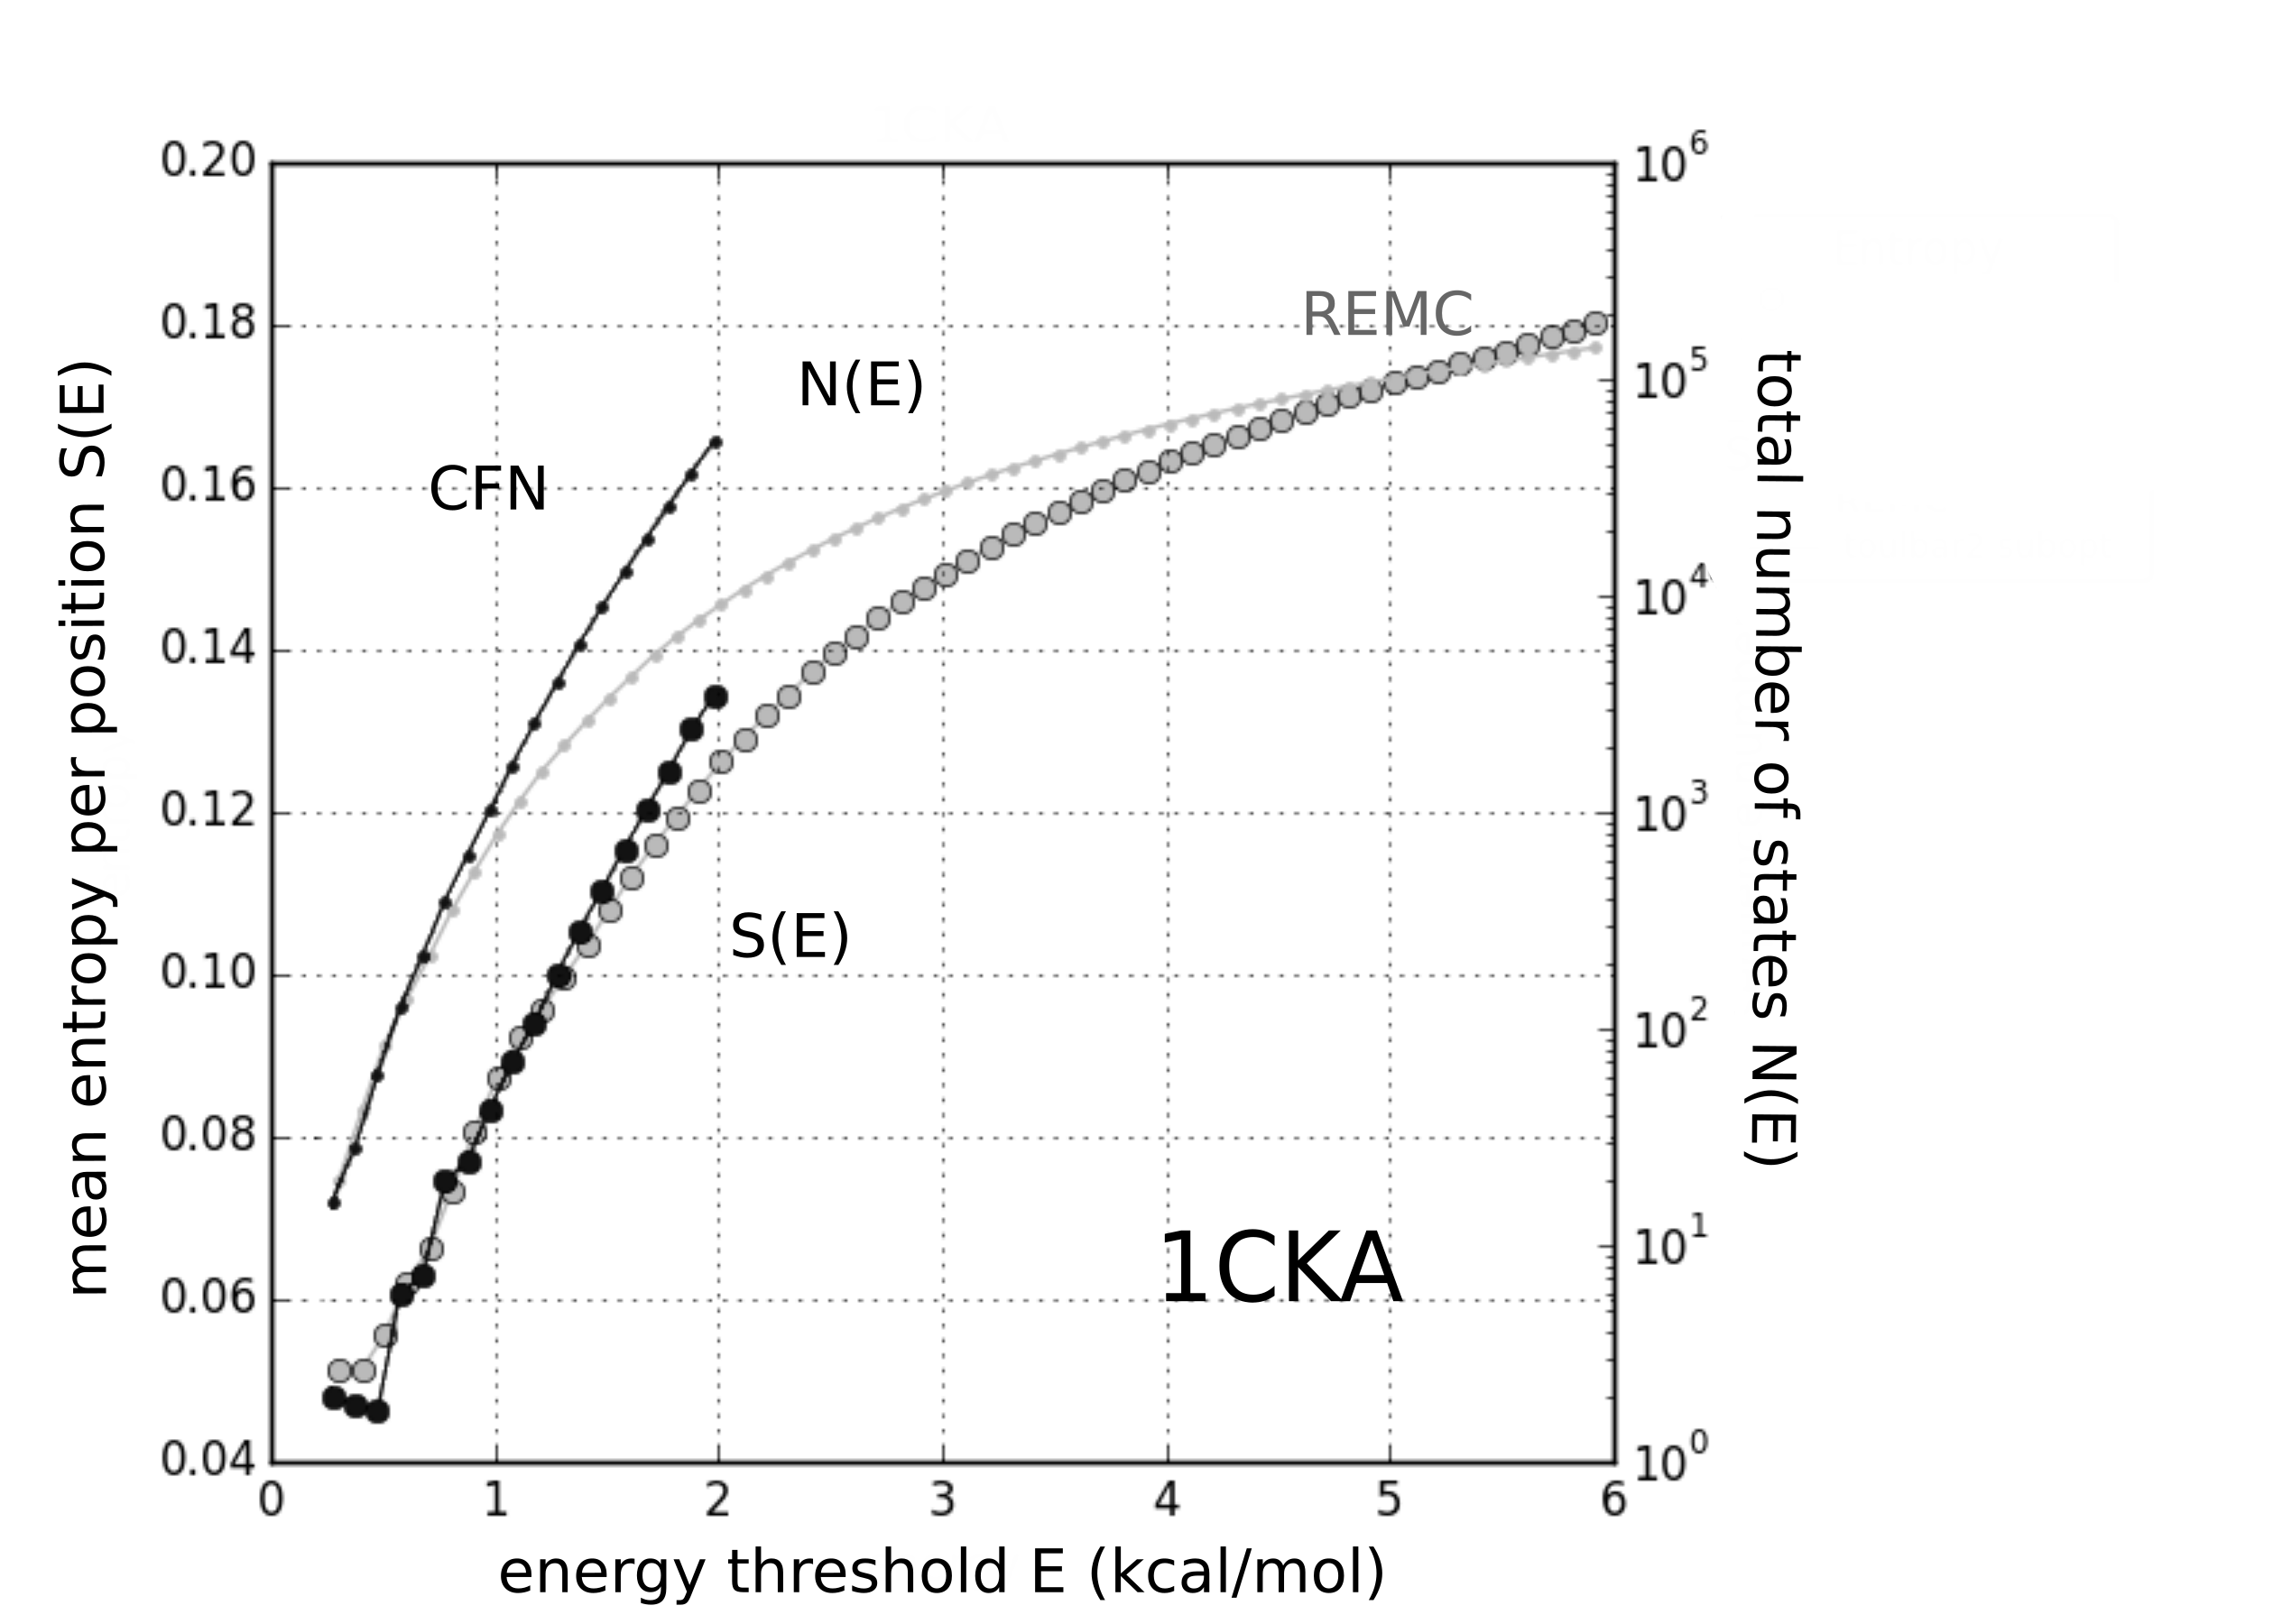
\includegraphics[trim = 0mm 0mm 25mm 0mm, clip,width=12cm]{1CKA_entropy_seqnb.png} 
\caption{ 
Sequence entropy $S(E)$ and number of states $N(E)$ within a given energy range $E$ above the GMEC for the 1CKA SH3 domain. Ten positions were allowed to vary. The entropy (large dots) is a single position sequence entropy, Eq.\ (\ref{eq:entropy}), averaged over all the variable positions. CFN results (black) are based on a complete enumeration of all states within the energy range (at most $E$ kcal/mol above the GMEC). REMC results (gray) are based on the states sampled by all eight walkers during a single trajectory. The number of states (small dots) corresponds to all the different combinations of sequences and rotamers.
}
       \label{fig:entropy}
    \end{figure}

However, the REMC diversity at each position agrees very well with the CFN result up to about 1.5 kcal/mol above the GMEC. At $E$ = 2 kcal/mol above the GMEC, the REMC entropy is still 93\% of the exact value.
Thus, REMC samples the full sequence diversity at each position in this range, even though it does not sample exhaustively all the combinations of mutations (let alone rotamers) at all positions. Thus, for any pair of positions, REMC may not sample all combinations of allowed amino acid classes (up to 25 combinations, since the allowed sidechain types are grouped into five classes; see Methods) but it effectively samples, at either position, the same types as the exact method.

As we consider higher energy threshold values, $E$ $\ge$ 3 kcal/mol, the number of states sampled by REMC increases exponentially and the entropy increases in a quasilinear way. Different replicas sample different energy ranges, as expected; for example, the $kT$=0.592 and $kT$=0.888 kcal/mol replicas sample the 4--10 and 11--14 kcal/mol ranges, respectively. 

\section{Concluding Discussion}
Stochastic search methods are very common in CPD. They often take the form of MC-based simulated anealing (SA) [1, 58]; various forms of biased or quenched Monte Carlo are also popular [59, 61–63]. For example, MC moves can be chosen to preferentially affect residues that have a high local energy [62] and/or selected degrees of freedom can be subjected to energy minimization (quenched) during or after an MC move. The steepest-descent heuristic used here [32] has similarities to quenched MC. These particular quenched or biased stochastic methods do not sample a Boltzmann distribution of states, but aim to be as effective as possible at identifying low energy sequences, including the GMEC. They can be extended to very large search spaces that include backbone flexibility [64–66], and they do not directly depend on additive energy functions (although additivity can dramatically increase efficiency). In contrast, while exact methods like CFN have been extended beyond discrete rotamer sets [21, 67], and can handle slight departures from a purely additive energy function (ones including 3- or 4-body energy terms) [68, 69], they cannot readily handle arbitrary energy functions or a flexible backbone. Other stochastic methods preserve the Boltzmann character of the statistical ensemble, including plain Monte Carlo, Replica Exchange MC, and configuration bias MC methods [28, 58]. At the same time, REMC benefits from high temperature sampling, like simulated annealing, with energy ranges of 10 kcal/mol or more above the GMEC readily accessible in this work.
Here, we tested three stochastic search methods, and compared their ability to identify low energy sequences in problems of increasing size/complexity. While the capability to identify the low energy sequences is important, we should keep in mind that their significance is only as good as the energy function, as illustrated above for 1A81. Direct comparison to the exact GMEC was possible routinely for problems involving up to 10 designed positions, and for 28 of 45 tests with 20 designed positions. The 10-position designs involved total rotamer numbers of 2500--3000; for the 20- and 30-position designs, there are about 2000 and 4000 more rotamers, respectively.
The larger tests are relevant for whole protein design projects, as well as projects that redesign one or more large protein surfaces (eg, protein crystal design). For these tests, the GMEC was usually not available, despite using a very recent Toulbar2 protocol \cite{Simoncini15} .
Therefore, the stochastic methods could only be evaluated indirectly.
The indirect quality indicators were  (a) consistency between the methods and (b) general sequence quality compared to experiment. Agreement between the heuristic and REMC solutions was very good in general, and agreement with experimental Pfam sequences was excellent for core residues, as observed previously with the same energy function (but a heuristic exploration method) \cite{Schmidt09,Schmidt10}. Results with a more advanced protein force field and Generalized Born solvent are expected to be even better \cite{Polydorides11,Simonson15a}.
Designed surface residues were less similar to experiment, which can be partly explained because the experimental sequences are subject to additional constraints and selective pressures (such as domain-domain interactions), not included in the design.  

Overall, the heuristic and REMC methods gave very good agreement with each other and with the GMEC when available, except for some of the whole-protein design tests.
CFN, in its Toulbar2 implementation was very effective for up to 10 designed positions. Exploration speed was similar for all methods for 10-position design, and similar for the stochastic methods applied to the larger problems. With 8-walker REMC and 0.75 billion steps per walker, the three largest departures from the overall best energy, among 67 large, difficult tests, were 4, 3, and 2.4 kcal/mol.
Sequence diversity was also recapitulated accurately, compared to exact enumeration, in the very limited range where the latter was possible.
In addition, REMC sampled suboptimal solutions as much as 10 kcal/mol above the GMEC, providing thermal averages and an approximate solution to the inverse folding problem.
We have recently extended the REMC method to allow backbone moves, with the help of a hybrid move scheme to be described elsewhere.
Overall, both the heuristic and REMC method appear to be effective search and sampling methods for most problems and problem sizes.

\clearpage
\pagebreak



%%% Local Variables:
%%% mode: latex
%%% TeX-master: "../these"
%%% End:

